\documentclass[11pt]{article}

\usepackage[portuguese]{babel}
\usepackage[utf8]{inputenc}
\usepackage{amsmath}
\usepackage{graphicx}
\usepackage{float}
\usepackage{subfig}
\usepackage{fixltx2e}
\usepackage[bottom]{footmisc}
\usepackage{color}
\usepackage{xargs}                      % Use more than one optional parameter in a new commands
\usepackage[pdftex,dvipsnames]{xcolor}  % Coloured text etc.
\usepackage[colorinlistoftodos,prependcaption,textsize=tiny]{todonotes}
\newcommandx{\unsure}[2][1=]{\todo[linecolor=red,backgroundcolor=red!25,bordercolor=red,#1]{#2}}
\newcommandx{\change}[2][1=]{\todo[linecolor=blue,backgroundcolor=blue!25,bordercolor=blue,#1]{#2}}
\newcommandx{\info}[2][1=]{\todo[linecolor=OliveGreen,backgroundcolor=OliveGreen!25,bordercolor=OliveGreen,#1]{#2}}
\newcommandx{\improvement}[2][1=]{\todo[linecolor=Plum,backgroundcolor=Plum!25,bordercolor=Plum,#1]{#2}}
\newcommandx{\thiswillnotshow}[2][1=]{\todo[disable,#1]{#2}}
\usepackage[font=footnotesize]{caption}

\numberwithin{equation}{section}

\linespread{1.3}
\usepackage{indentfirst}
\usepackage[top=2cm, bottom=2cm, right=2.25cm, left=2.25cm]{geometry}
\addto\captionsportuguese{\renewcommand{\contentsname}{Índice}}

\begin{document}

\begin{titlepage}
\begin{center}

\hfill \break
\hfill \break


\includegraphics[width=0.3\textwidth]{./logo}~\\[1cm]

\textsc{\LARGE Instituto Superior Técnico}\\[0.25cm]
\textsc{\Large Mestrado Integrado em Engenharia Electrotécnica e de Computadores}\\[1.8cm]
\textsc{\huge Sistemas Integrados Analógicos}\\[0.25cm]

{\huge \bfseries \textit{Design} de um Amplificador \\[1cm]}

\begin{tabular}{ l l }
João Bernardo Sequeira de Sá & \hspace{2mm} n.º 68254 \\
Maria Margarida Dias dos Reis & \hspace{2mm} n.º 73099 \\
Nuno Miguel Rodrigues Machado & \hspace{2mm} n.º 74236
\end{tabular}

\vfill

{\large Lisboa, 31 de Maio de 2015} 

\end{center}
\end{titlepage}

\pagenumbering{gobble}
\clearpage

\tableofcontents
\pagebreak

\clearpage
\pagenumbering{arabic}

\section{Introdução}

Pretende-se projectar um amplificador \textit{folded cascode} CMOS OTA de dois andares de acordo com as especificações da seguinte tabela.

\begin{table}[H]
	\centering
	\caption{Características do amplificador a projectar.}
	\vspace{-1.5mm}
	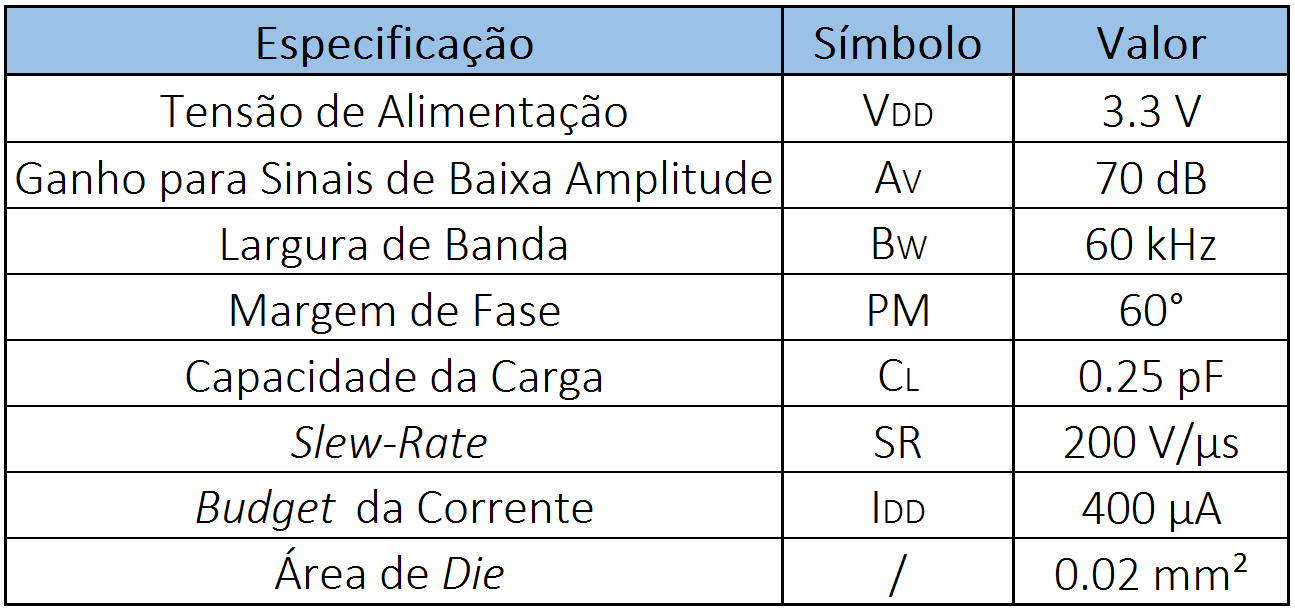
\includegraphics[keepaspectratio=true, scale=0.45]{teoricas/tabela1}
	\label{tab:tab1}
\end{table}

O circuito de ponto de partida para a realização do projecto é apresentado de seguida.

\begin{figure}[H]
	\centering
	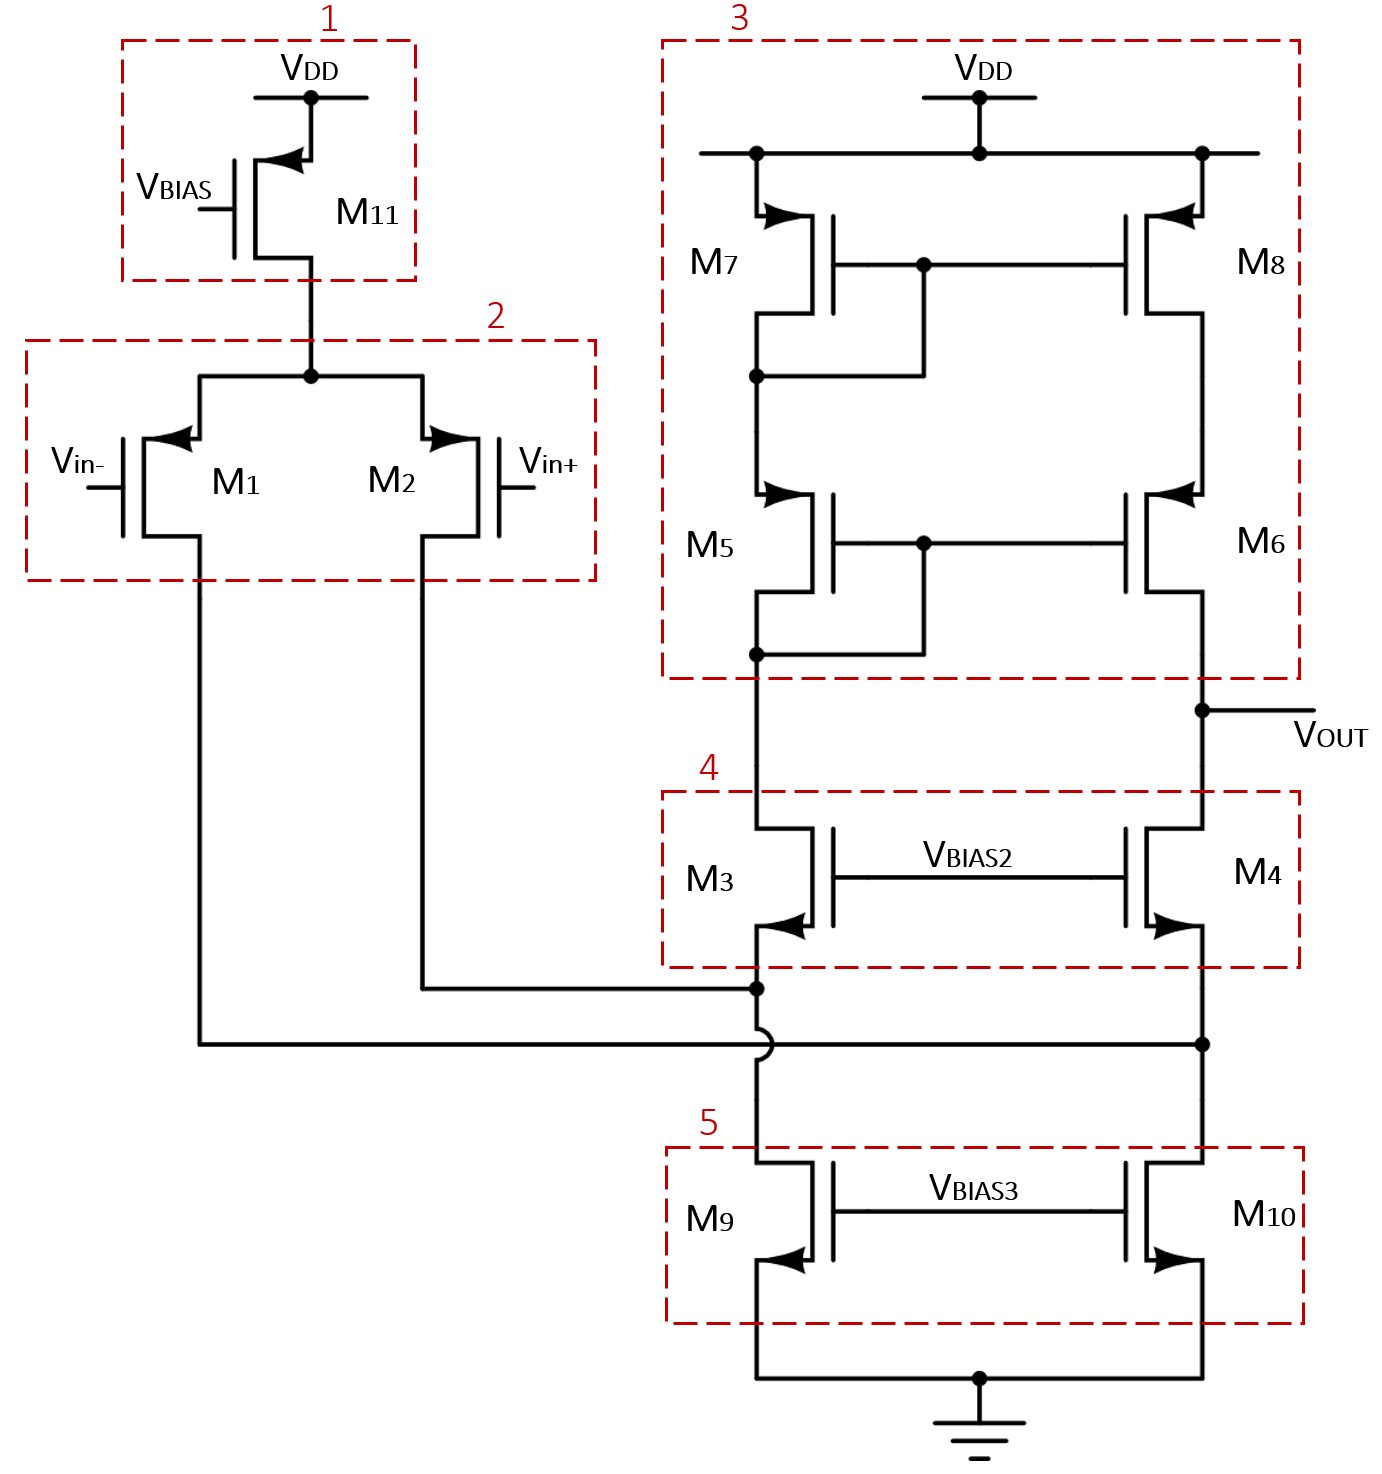
\includegraphics[keepaspectratio=true, scale=0.50]{teoricas/circuito1}
	\vspace{-0.5em}
	\caption{Circuito do amplificador a projectar.}
	\vspace{-0.8em}
\end{figure} 

\section{Adenda ao \textit{Middle Target}}

Esta secção foi acrescentada ao relatório final no intuito de corrigir os resultados obtidos e apresentados no relatório anterior, o do \textit{middle target}. Como referenciado, pretende-se projectar um amplificador \textit{folded cascode} CMOS OTA de dois andares de acordo com as especificações da Tabela \ref{tab:tab1}.

\subsection{Detecção dos erros} 

Foram identificados vários erros no relatório intermédio que comprometem os resultados apresentados anteriormente. A primeira correcção foi referente ao \textit{schematic} do \textit{testbench} que permite simular o circuito em testes de resposta AC. Foi colocado um \textit{switch} que simula a bobine - provoca um circuito aberto para um regime AC e curto-circuito para um regime DC. Foi também alterada a amplitude do sinal de entrada de 3.3 V para 1.6 V, sendo que esta alteração garante que os transístores não saem da saturação. De seguida pode-se comparar o novo \textit{testbench} com o anterior.

\begin{figure}[H]
	\centering
	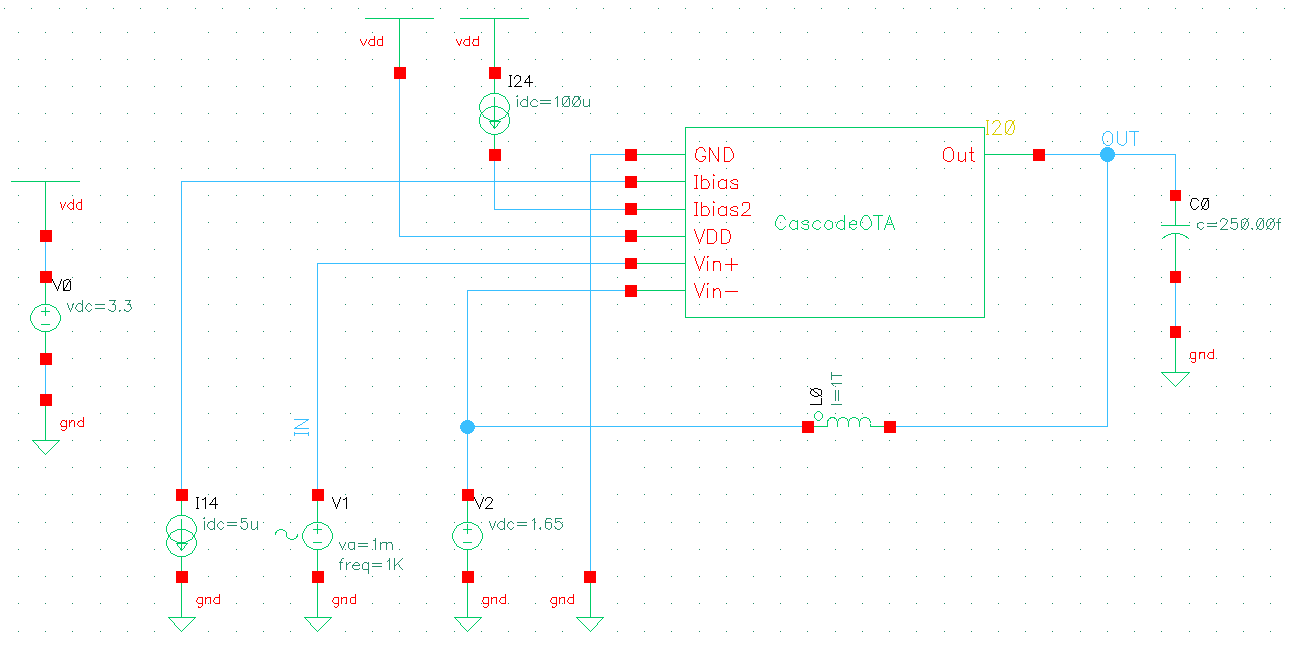
\includegraphics[keepaspectratio=true, scale=0.60]{exps/TBac}
	\vspace{-0.5em}
	\caption{\textit{Schematic} do \textit{testbench} anterior que permite simular o circuito em testes de resposta AC.}
	\vspace{-0.8em}
\end{figure} 

\begin{figure}[H]
	\centering
	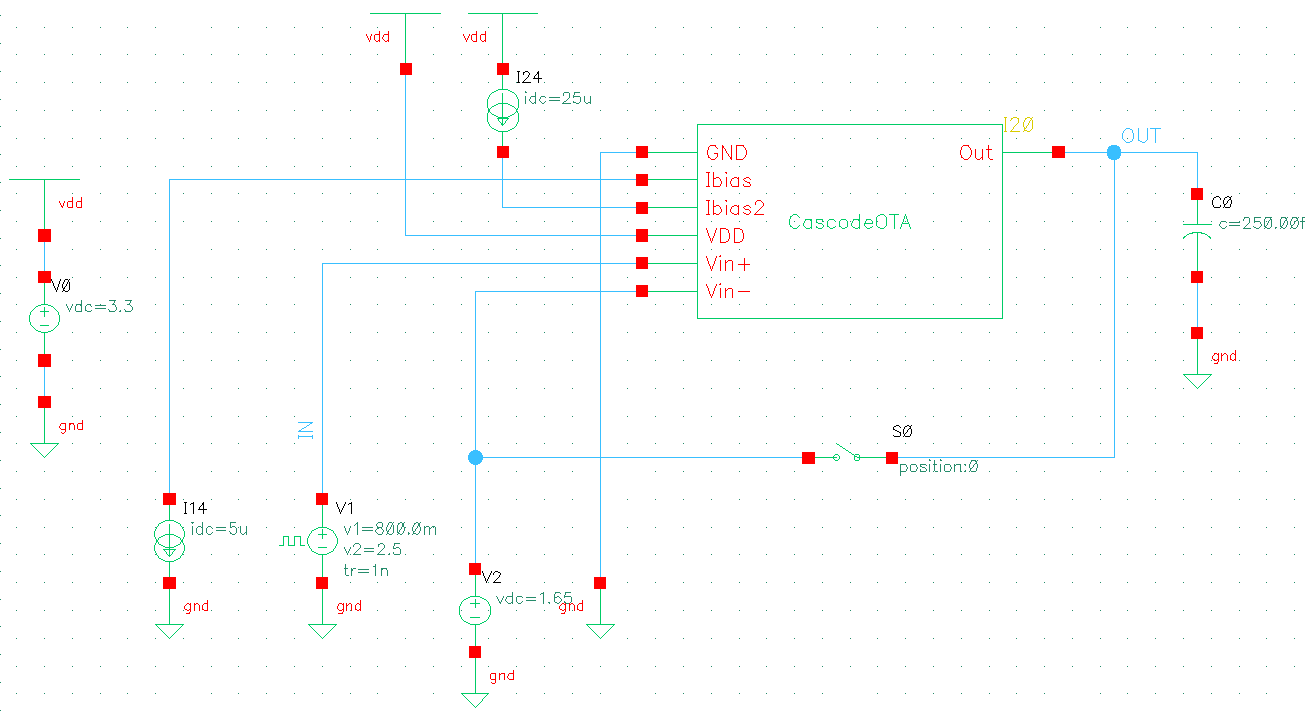
\includegraphics[keepaspectratio=true, scale=0.50]{exps/testebenchantigo}
	\vspace{-0.5em}
	\caption{\textit{Schematic} do novo \textit{testbench} que permite simular o circuito em testes da \textit{slew-rate} e de resposta transiente, DC e AC.}
	\vspace{-0.8em}
\end{figure} 

Outro erro identificado é referente ao cálculo da \textit{slew-rate}. No relatório intermédio, o resultado da \textit{slew-rate} era relativo só ao flanco de descida, sendo necessário demonstrar para os dois flancos - subida (equação 2.1) e descida (equação 1.2). 

\vspace{-3mm}
\begin{equation}
	\text{slewRate} (\text{VT("/OUT")} \:\: 1 \:\: \text{nil} \:\: 2 \:\: \text{nil} \:\: 10 \:\: 90 \:\: \text{nil} \:\: "\text{time}")
\end{equation}

\vspace{-3mm}
\begin{equation}
	\text{slewRate} (\text{VT("/OUT")} \:\: 2 \:\: \text{nil} \:\: 1 \:\: \text{nil} \:\: 10 \:\: 90 \:\: \text{nil} \:\: "\text{time}")
\end{equation}

A equação \texttt{slewRate} é obtida com recurso à calculadora do Cadence, escolhendo o sinal pretendido, que, neste caso, é a saída do \textit{cascode} OTA, \texttt{VT("/OUT")}. De seguida escolhe-se a posição inicial e final para o cálculo da \textit{slew-rate} - foi definido que para o flanco de descida começa-se a calcular desde 2 V até 1 V e no flanco de subida o cálculo é o inverso, de 1 V até 2 V. O intervalo anteriormente referido foi escolhido de forma a calcular a \textit{slew-rate} na zona onde os transístores se encontram na saturação.

\subsection{Correcção do dimensionamento}

Com os erros anteriormente referidos corrigidos, o circuito apresentado na entrega intermédia falhava em algumas especificações: ganho para sinais de baixa amplitude, margem de fase e largura de banda. Na secção seguinte apresenta-se os resultados das simulações de Monte Carlo e \textit{corners}.

Com o intuito de corrigir as dimensões, partiu-se de um critério inicial - obter transístores de dimensões mais reduzidas e manter o rácico $W/L$ obtido no relatório anterior. Em primeiro lugar, verificou-se que com a nova expressão do cálculo da \textit{slew-rate} obtém-se valores mais elevados, o que significa que se pode reduzir as dimensões dos transístores M\textsubscript{9} e M\textsubscript{10}. 

De seguida pretendeu-se melhorar a margem de fase e, analisando o resultado das especificações pretendidas, verificou-se que era necessário aumentar a largura de banda de forma a obter uma margem de fase melhor sem alterar significativamente os resultados das outras especificações. Começou-se por analisar as dimensões das capacidades do circuito e verificou-se que a capacidade referente aos transístores M\textsubscript{7} e M\textsubscript{8} é a capacidade que mais influencia a margem de fase. Mas, como já foi referido no relatório anterior, os transístores M\textsubscript{7} e M\textsubscript{8} também afectam o ganho e a largura de banda, como se pode ver pelas expressões seguintes. 

\vspace{-3mm}
\begin{equation}
A_{v} = g_{m_1} R_o =  g_{m_1}\left[\left(g_{m_4}r_{o_4}\left(r_{o_2}//r_{o_{10}}\right)\right)//\left(g_{m_6}r_{o_6}r_{o_8}\right)\right];
\end{equation}
\vspace{-2mm}
\begin{equation}
f_{p} = \frac{1}{2\pi C_L R_o} = \frac{1}{2\pi C_L \left[\left(g_{m_4}r_{o_4}\left(r_{o_2}//r_{o_{10}}\right)\right)//\left(g_{m_6}r_{o_6}r_{o_8}\right)\right]};
\end{equation} 

\vspace{2mm}
Assim sendo, e analisando as expressões decidiu-se inicialmente diminuir as dimensões dos transístores M\textsubscript{7} e M\textsubscript{8}, o que fez aumentar a largura de banda como também a margem de fase. Com o intuito de melhorar as especificações obtidas diminui-se as dimensões dos transístores M\textsubscript{3} e M\textsubscript{4} até atingir uma dimensão de $L$ miníma de 0.85 $\mu$m. Como a dimensão $L$ dos transístores M\textsubscript{5} e M\textsubscript{6} é menor que 0.85 $\mu$m, aumentou-se as dimensões com o intuito de manter o critério de um L mínimo de 0.85 $\mu$m.

Com estas alterações consegui-se obter todas a especificações excepto para o ganho de sinais de baixa amplitude. Analisando a expressão anterior do ganho, verifica-se que para aumentar o ganho sem alterar as restantes especificações, seria necessário aumentar o valor de $g_{m_1}$. Como o valor de $g_m$ é directamente proporcional a $I_D$, com aumento de $W$ existe um aumento de $I_D$ e de $g_m$. A expressão seguinte mostra como $W$ influencia $I_D$:

\vspace{-3mm}
\begin{equation}
g_{m} \propto I_{D}= k_P \times \left(\frac{W}{L}\right) \times V_{OD}^2 \times \left(1+\lambda V_{DS}\right).
\end{equation}

Para aumentar o $g_{m_1}$ é necessário alterar o rácio $W/L$, ou seja, o rácio de M\textsubscript{1} e M\textsubscript{2} sofreu um aumento de 132\%, passando de 43 para 100. Não é preocupante esta alteração do valor da transcondutância, não se comprometendo a zona de funcionamento dos transístores pois estes são polarizados externamente.

\todo{explicar as polarizacoes com que ficamos - 13uA e 29uA}

Assim, o circuito final relativamente à entrega intermédia é:

\begin{figure}[H]
	\centering
	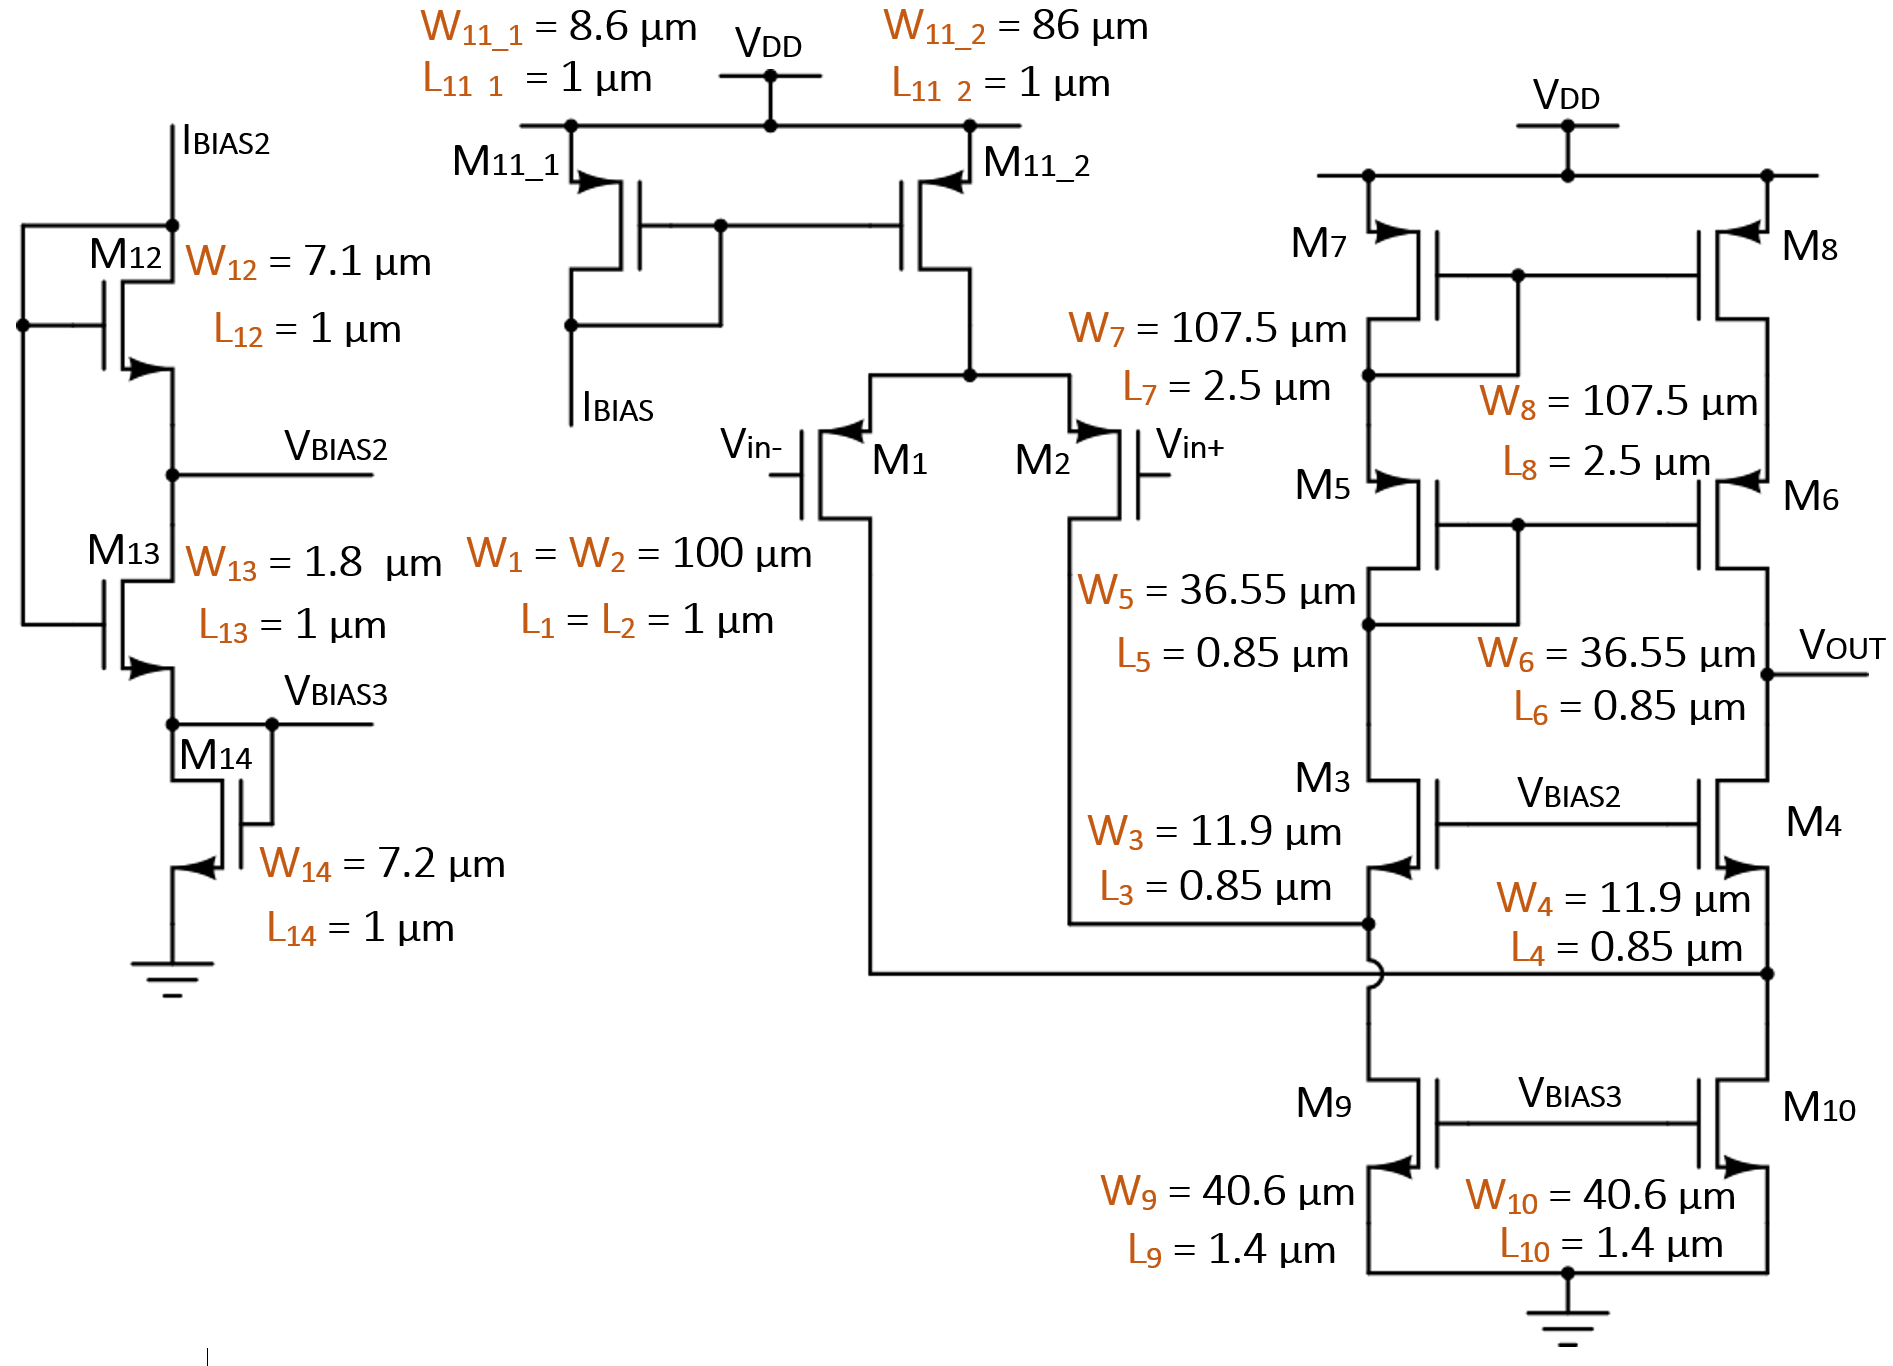
\includegraphics[keepaspectratio=true, scale=0.42]{teoricas/circuitoantesdadiv}
	\vspace{-0.5em}
	\caption{Circuito final da entrega intermédia.}
	\vspace{-0.8em}
	\label{fig:finalint}
\end{figure} 

\begin{table}[H]
	\centering
	\caption{Dimensões dos transístores que constituem o amplificador.}
	\vspace{-1.5mm}
	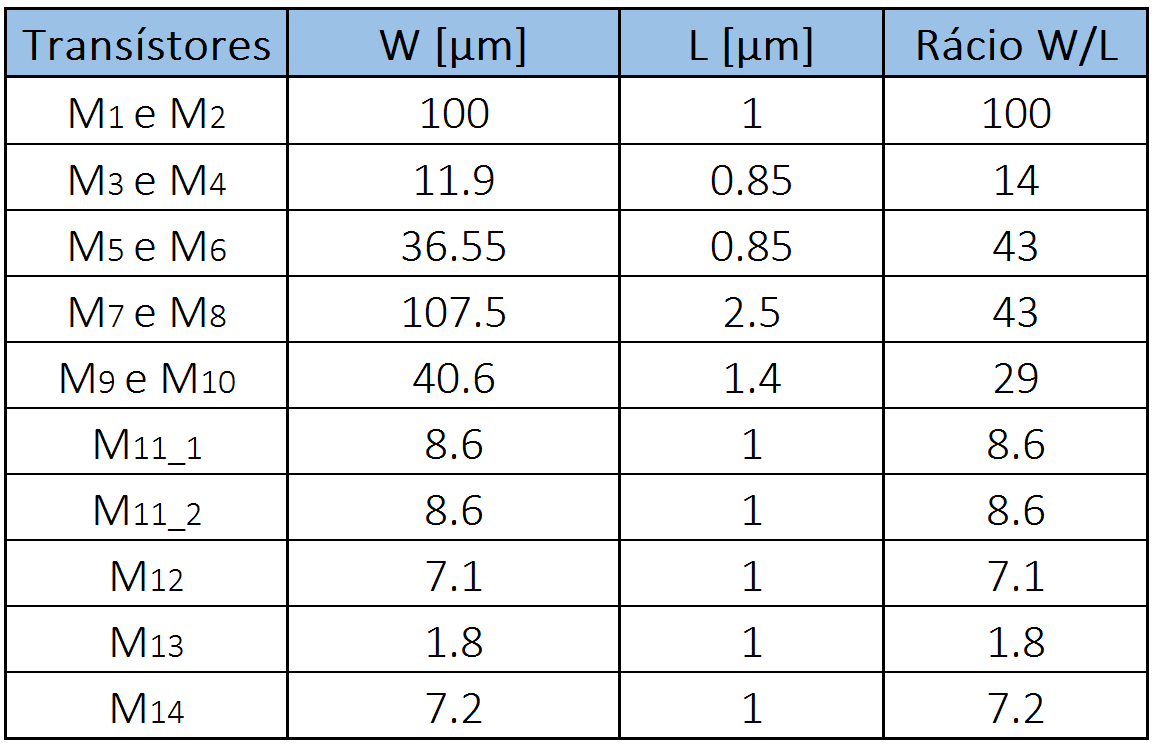
\includegraphics[keepaspectratio=true, scale=0.35]{teoricas/dimensoes1}
\end{table}

Com este circuito as especificações finais obtidas para o circuito com recurso à simulação da Figura 3 são apresentadas na seguinte tabela.

\begin{figure}[H]
	\centering
	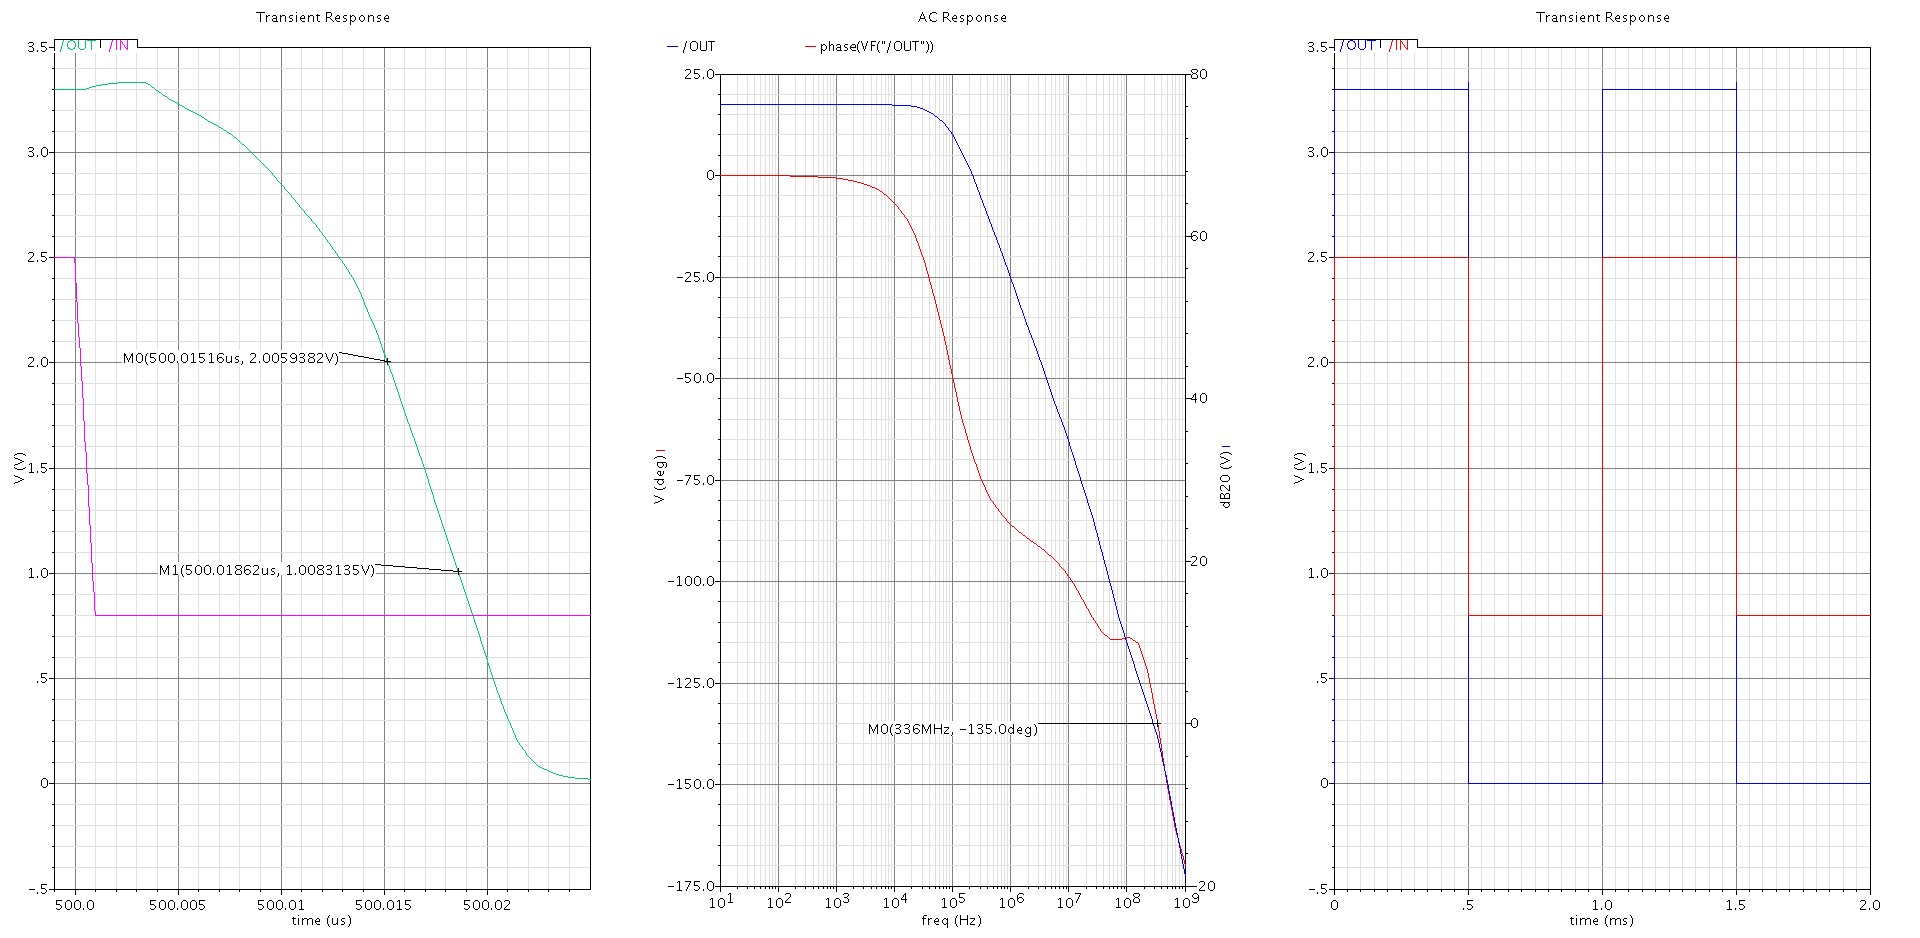
\includegraphics[keepaspectratio=true, scale=0.25]{exps/SIngle_Run}
	\vspace{-0.5em}
	\caption{Simulações efectuadas com o circuito final do \textit{middle target}.} 
	\vspace{-0.8em}
\end{figure} 

Relativamente às especificações que se pretende apresenta-se de seguida uma tabela com um resumo.

\begin{table}[H]
	\centering
	\caption{Especificações obtidas com o circuito final do \textit{middle target}.}
	\vspace{-1.5mm}
	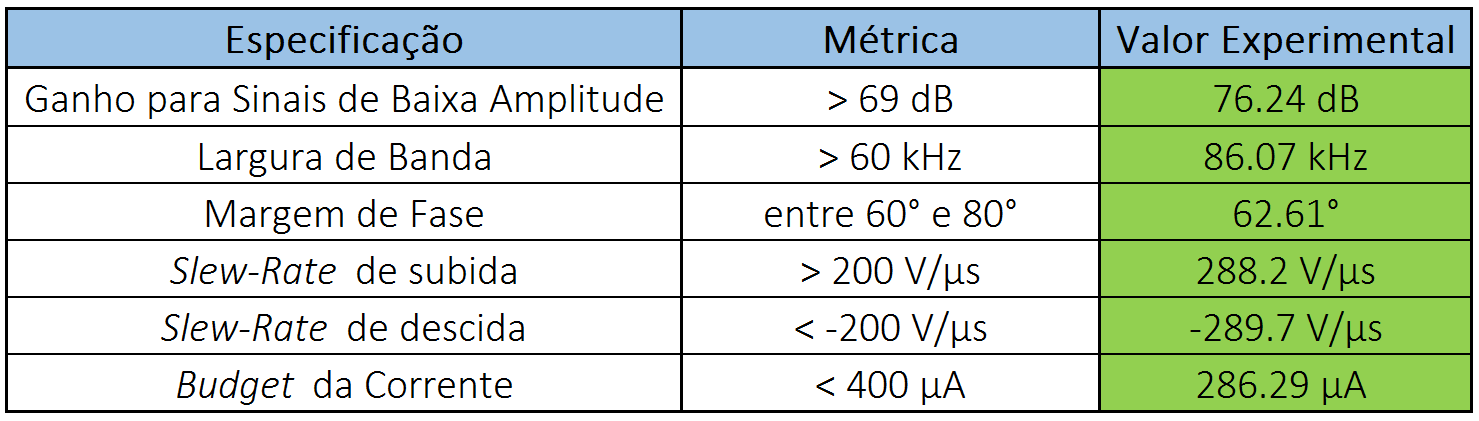
\includegraphics[keepaspectratio=true, scale=0.35]{teoricas/specsfinal}
\end{table}

\subsection{Demonstração de resultados} 

Nesta secção apresenta-se os resultados do dimensionamento do relatório intermédio e do novo dimensionamento anteriormente referido, para simulações de Monte Carlo e de \textit{corners}.

\subsubsection{Resultados do dimensionamento inicial} 

\begin{figure}[H]
	\centering
	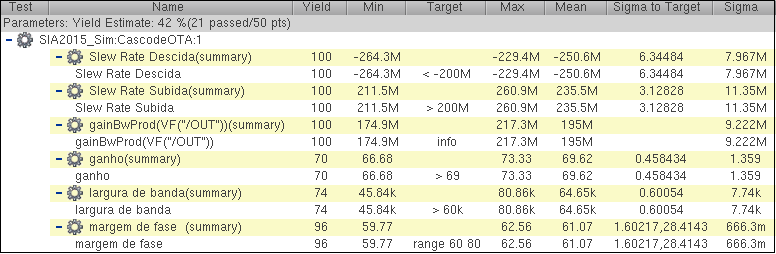
\includegraphics[keepaspectratio=true, scale=0.65]{exps/MonteCarlo_50pt_Antigo}
	\vspace{-0.5em}
	\caption{Simulação de Monte Carlo para 50 pontos.}
	\vspace{-0.8em}
\end{figure} 

\begin{figure}[H]
	\centering
	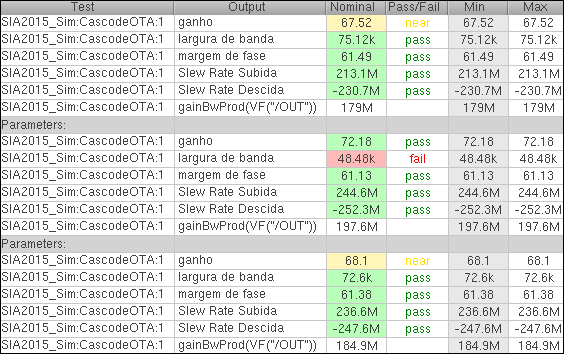
\includegraphics[keepaspectratio=true, scale=0.65]{exps/MonteCarlo_3pt_Antigo}
	\vspace{-0.5em}
	\caption{Resultados obtidos para as 3 primeiras simulações de Monte Carlo.}
	\vspace{-0.8em}
\end{figure} 

\begin{figure}[H]
	\centering
	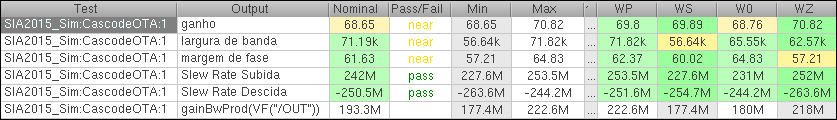
\includegraphics[keepaspectratio=true, scale=0.65]{exps/Corners_Antigo}
	\vspace{-0.5em}
	\caption{Simulação por \textit{corners}.}
	\vspace{-0.8em}
\end{figure} 

Tal como se pode observar das tabelas de resultados, antes das correções obtinha-se um \textit{yeld} de 70\%, ou seja em cada 4 \textit{batches} pelo menos um não seria utilizável. Estas falhas eram maioritariamente devidas ao ganho e à largura de banda, pelo que tal como se referiu anteriormente foi especialmente aí que incidiram as correcções feitas. Tem-se também uma falha minima na margem de fase levando a um \textit{yeld} de 96\% que seria aceitável. Tem-se também que a simulação por \textit{corners} não apresenta os resultados desejados, sendo que novamente o ganho a largura de banda apresentam os piores resultados com a margem de fase também a ter falhas.

\subsubsection{Resultados do dimensionamento corrigido} 

\begin{figure}[H]
	\centering
	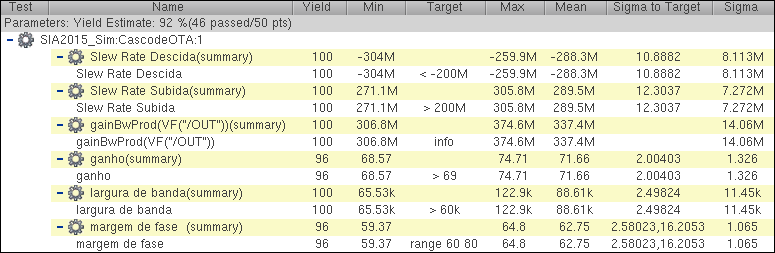
\includegraphics[keepaspectratio=true, scale=0.65]{exps/MonteCarlo_50pt_Novo}
	\vspace{-0.5em}
	\caption{Simulação de Monte Carlo para 50 pontos.}
	\vspace{-0.8em}
\end{figure} 

\begin{figure}[H]
	\centering
	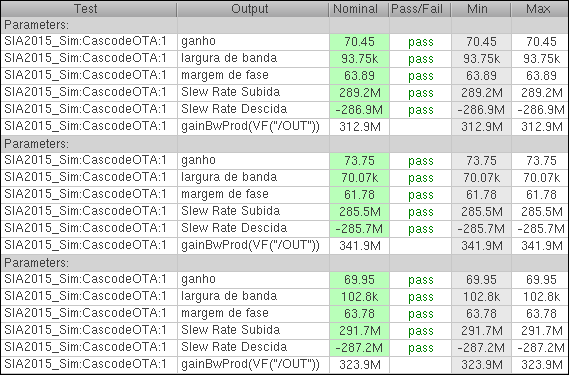
\includegraphics[keepaspectratio=true, scale=0.65]{exps/MonteCarlo_3pt_Novo}
	\vspace{-0.5em}
	\caption{Resultados obtidos para as 3 primeiras simulações de Monte Carlo.}
	\vspace{-0.8em}
\end{figure} 

\begin{figure}[H]
	\centering
	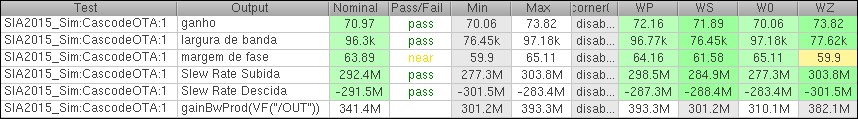
\includegraphics[keepaspectratio=true, scale=0.65]{exps/Corners_Novo_semDiv}
	\vspace{-0.5em}
	\caption{Simulação por \textit{corners}.}
	\vspace{-0.8em}
\end{figure} 

Após as correções os resultados são muito mais positivos, estando dentro dos requisitos do \textit{target}. O \textit{yeld} final é de 96\% para 50 \textit{runs}, que se considera um resultado bastante aceitável. Considerou-se um valor de ganho inferior ao do \textit{target} com o valor de 69 dB. Esta consideração é permitida pois obteve-se um produto de ganho largura de banda superior ao do \textit{target} nos casos em que não se obteve os 70 dB desejados pelo que ao aplicar realimentação se pode aumentar o ganho à custa de largura de banda, ficando-se dentro dos parâmetros desejados.
Na simulação por \textit{corners} obteve-se também resultados aceitáveis, sendo a única falha na margem de fase, com um erro de cerca de 1\%. 

\section{Projecção do \textit{Layout}}

\subsection{Multiplicidade e \textit{Fingers}}

Para projectar o \textit{layout} do circuito da Figura \ref{fig:finalint} optou-se por dividir os transístores de grandes dimensões com recurso a duas técnicas - multiplicidade e \textit{fingers}. A técnica de \textit{fingers} corresponde a um arranjo específico do transístor com $n$ \textit{gate fingers} em que as difusões da \textit{source} e do \textit{drain} são partilhadas. Se se tiver $n$ \textit{fingers} haverá então $n+1$ difusões. A multiplicidade é quando se faz uma ligação em paralelo de múltiplos dispositivos MOS, sendo que o agregado deles corresponde a um só transístor. Observa-se também que utilizar \textit{fingers} reduz a capacidade do transístor, aproximando-a da capacidade linear, sendo especialmente importante nos casos que afectem a largura de banda e margem de fase. 

Do ponto de vista da definição correspondem ao mesmo, mas são de facto duas maneiras diferentes de pensar na paralelização de transístores. Com o recurso a \textit{fingers} tem-se uma única célula com o transístor completo com todos os \textit{fingers}, útil para quando se quer uma célula mais compacta, enquanto na multiplicidade tem-se tantos transístores quanto a multiplicidade indicar. De facto, é possível conjugar as duas técnicas, ou seja, cada dispositivo MOS da multiplicidade pode ser feito com vários \textit{fingers}.

Para o trabalho em causa optou-se por usar as duas técnicas teoricamente idênticas para adquirir mais experiência e para verificar as diferenças que têm ao nível de implementação prática no Cadence.

Estas práticas são aplicadas também de forma a evitar  efeitos nocivos de \textit{mismatches}, ou seja da vulnerabilidade aos gradientes de parâmetro. Ao minimizar a área efectiva dos circuitos protege-se assim o dispositivo destes efeitos.

Sendo assim deu-se especial atenção aos pares de transístores em que se considerou que existe uma maior sensibilidade a \textit{mismatches}. São este os pares M\textsubscript{1}/M\textsubscript{2}, M\textsubscript{7}/M\textsubscript{8}, M\textsubscript{9}/M\textsubscript{10} e M\textsubscript{11\textsubscript{1}}/M\textsubscript{11\textsubscript{2}}. 

Começou-se em primeira instância por aplicar multiplicidade, tentando aproximar ao máximo os tamanhos dos pares que estão ligados entre si, seguido de uma redução geral dos transístores de todo o circuito. 

Em adição a multiplicidade optou-se por usar também a técnica \textit{fingers} no par M\textsubscript{7}/M\textsubscript{8} pois este par, tal como já foi mencionado, tem grande influencia na largura de banda e margem de fase. Já no par \textsubscript{5}/M\textsubscript{6} aplicou-se apenas a técnica \textit{fingers} ficando-se assim com tamanhos da mesma ordem em ambos os pares para além de uma forma compacta facilitando as tarefas de escolher uma disposição para os transístores e efectuar as ligações internas.

Como o rácio de espelhamento é muito sensível a diferenças nos parâmetros do espelho de corrente, ou seja a\textit{mismatches}, nos pares de transistores M\textsubscript{11\textsubscript{1}}/M\textsubscript{11\textsubscript{2}}. Dado isto foi aplicada multiplicidade no transístor M\textsubscript{11\textsubscript{2}} de forma a que tivesse o mesmo tamanho que o M\textsubscript{11\textsubscript{1}} sendo assim o par afectado de igual forma pelos gradientes de parâmetros.

Para o par M\textsubscript{9}/M\textsubscript{10}, como são transístores NMOS e se optou por colocar num grupo apenas de NMOS, como será explicado à frente, houve apenas necessidade de reduzir os seus tamanhos através de multiplicidade para valores menos sensíveis a \textit{mismatches}.

Para os restantes cuja sensibilidade a variação de parâmetros não é tão importante quanto nos pares supramencionados usou-se multiplicidade de forma a obter-se as dimensões desejadas e também que facilitassem as estruturas do layout.

Assim, na tabela seguinte encontra-se uma descrição de como são constituídos os vários transístores do circuito.

\begin{table}[H]
	\centering
	\caption{Dimensões e características dos transístores do amplificador.}
	\vspace{-1.5mm}
	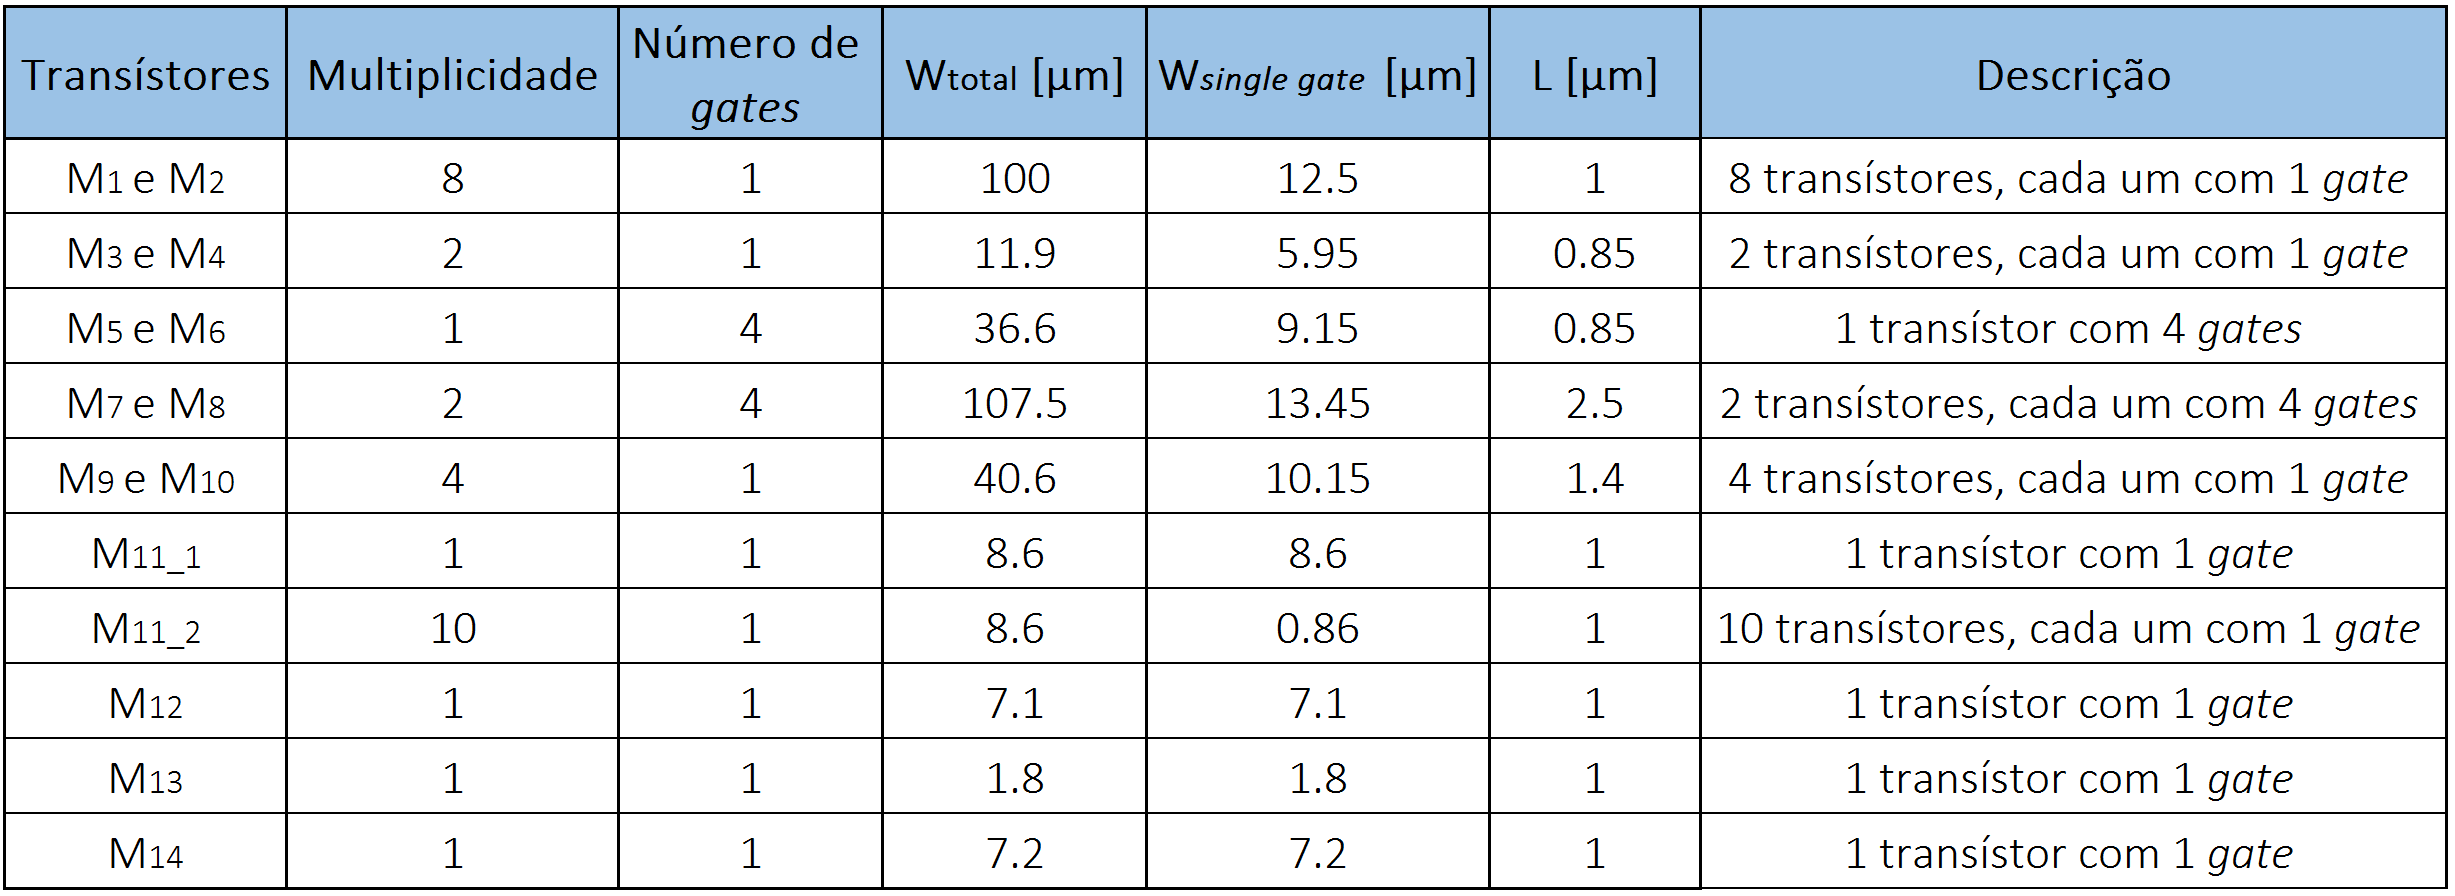
\includegraphics[keepaspectratio=true, scale=0.30]{teoricas/dimensoes2}
\end{table}

Após realizar as alterações comentadas anteriormente realizou-se novamente uma simulação Monte Carlo de forma a observar os seus efeitos. Apresenta-se assim o obtido na figura seguinte.

\begin{figure}[H]
	\centering
	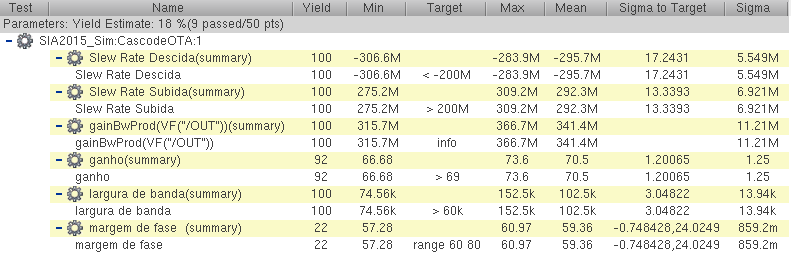
\includegraphics[keepaspectratio=true, scale=0.65]{exps/MonteCarlo_50pt_Novo_Sin}
	\vspace{-0.5em}
	\caption{Simulação Monte Carlo após aplicar técnicas de multiplicidade e \textit{fingers}.}
	\vspace{-0.8em}
\end{figure} 

Pode assim observar-se uma grande redução no \textit{yeld}, tendo-se obtido 22\%. Isto é devio em grande parte à margem de fase, sendo que existe ainda uma ligeira descida nos resultados do ganho, mas que ainda assim iria levar a \textit{yelds} aceitáveis. Esta influência na margem de fase deve-se a que ao utilizar multiplicidade aumenta-se o número de capacidades parasitas e a resistividade que aliado à fraca optimização do \textit{layout} produzido automaticamente pelo Cadence produz os resultados observados. Este problema será em grande parte resolvido com as práticas tomadas para realizar o \textit{layout} como se irá explicar nas secções seguintes, pois o intuito destas é especificamente para colmatar estes problemas.

\subsection{Disposição dos transístores}

Depois de se definir como estão estruturados os vários transístores é importante definir como se encontram dispostos no \textit{layout}. A topologia básica que foi utilizada é a de \textit{common centroid}. Através desta técnica consegue-se garantir um melhor \textit{matching} entre dois transístores iguais e em que se pretende um comportamento semelhante. De facto, o \textit{common centroid} é utilizado para se garantir que, e.g., um amplificador diferencial tenha um sinal de modo comum próximo de 0 e, como tal, um CMRR maior.

Para o circuito em causa foram definidos 4 blocos principais sobre os quais se definiu uma estrutura \textit{common centroid}:

\vspace{-2mm}

\begin{itemize}
	\item espelho de corrente básico que é polarizado em corrente com $I_{BIAS}$ (equivalente ao Bloco 1 da Figura 1) - estrutura \textit{common centroid} \#1;
	\vspace{-2mm}
	\item transístores do par diferencial (Bloco 2 da Figura 1) - estrutura \textit{common centroid} \#2;
	\vspace{-2mm}
	\item espelho de corrente cascode básico do tipo PMOS (Bloco 3 da Figura 1) - estrutura \textit{common centroid} \#3;
	\vspace{-2mm}
	\item transístores do tipo NMOS - estrutura \textit{common centroid} \#4;.
\end{itemize}

A escolha destes blocos foi feita com base no \textit{mismatch}. É essencial que entre os transístores do par diferencial não haja diferenças de comportamento, pois se houver o circuito fica desequilibrado. Os dois espelhos de corrente existentes também não devem ter \textit{mismatch}, pois pretende-se um espelhamento correcto. Como os transistores NMOS eram os mais pequenos e como não necessitam de estar dentro de um poço optou-se por juntar todos em apenas um bloco de forma a facilitar também a obtenção de \textit{common centroid} como será falado à frente.

De seguida apresenta-se as várias estruturas \textit{common centroid} definidas:

\begin{figure}[H]
	\centering
	\subfloat[]{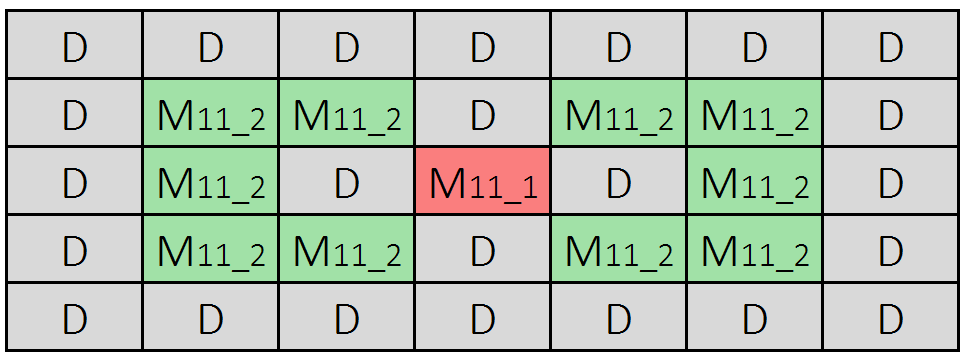
\includegraphics[keepaspectratio=true, scale=0.35]{teoricas/espelhodecorrente}}
	\hspace{8mm}
	\subfloat[]{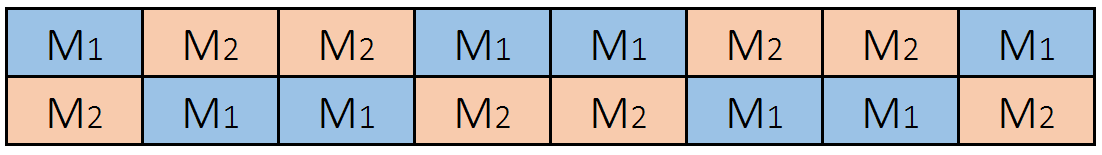
\includegraphics[keepaspectratio=true, scale=0.35]{teoricas/pardiferencial}}
	\linebreak
	\subfloat[]{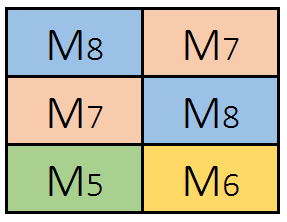
\includegraphics[keepaspectratio=true, scale=0.35]{teoricas/espelhodecorrenteamp}}
	\hspace{40mm}
	\subfloat[]{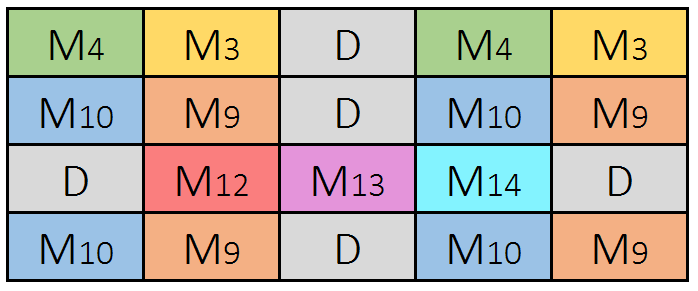
\includegraphics[keepaspectratio=true, scale=0.35]{teoricas/nmos}}
	\vspace{-0.8em}
	\caption{Estrutura \textit{common centroid} \#1 (a), \#2 (b), \#3 (c) e \#4 (d).}
	\vspace{-0.8em}
	\label{fig:common centroid}
\end{figure}

Nas figuras anteriores verifica-se a existências de transístores representados pela letra D - transístores \textit{dummies}. Este tipo de transístores serve para se garantir que os restantes transístores têm a mesma vizinhança, ou seja, que à sua volta vêem o mesmo. Veja-se o seguinte exemplo em que se consideram dois transístores - 1 e 2. O transístor 1 está definido com uma multiplicidade de 1 e o transístor 2 com uma multiplicidade de 8. Na figura seguinte encontra-se um exemplo de estrutura \textit{common centroid} para esse caso. 

\begin{figure}[H]
	\centering
	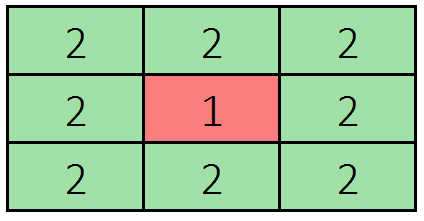
\includegraphics[keepaspectratio=true, scale=0.35]{teoricas/dummy1}
	\vspace{-0.5em}
	\caption{Exemplo de estrutura \textit{common centroid} com dois transístores.}
	\vspace{-0.8em}
\end{figure} 

O transístor 1 tem como vizinhança 4 transístores - para cima, para baixo, para a esquerda e para a direita. No entanto, qualquer transístor 2 tem uma ``falha'' naquilo que vê, pois não tem ``vizinhos'' nalgumas direcções. Assim, para se resolver este problema colocam-se transístores \textit{dummies} nos sítios onde há ``falhas''.

\begin{figure}[H]
	\centering
	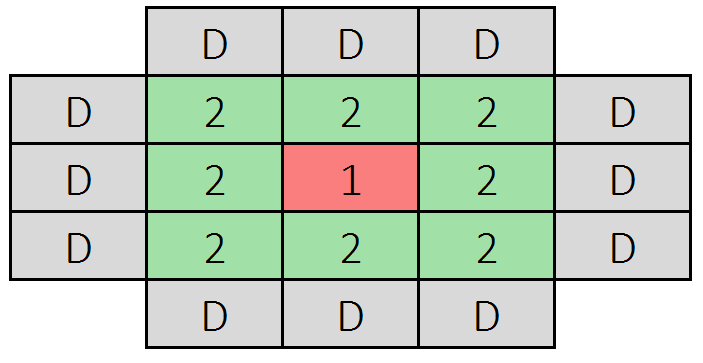
\includegraphics[keepaspectratio=true, scale=0.35]{teoricas/dummy2}
	\vspace{-0.5em}
	\caption{Exemplo de estrutura \textit{common centroid} com dois transístores e também transístores \textit{dummies}.}
	\vspace{-0.8em}
\end{figure}

De facto, os transístores \textit{dummies} não necessitam de ter as mesmas dimensões que os restantes e o circuito da figura anterior pode ser definido sa seguinte maneira.

\begin{figure}[H]
	\centering
	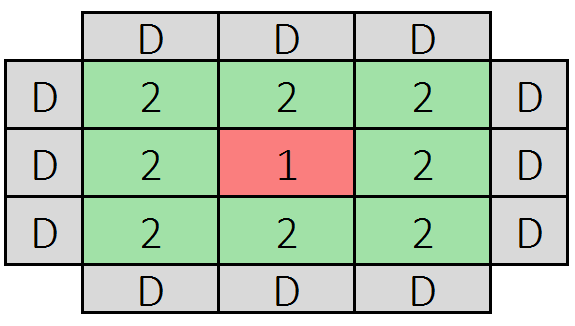
\includegraphics[keepaspectratio=true, scale=0.35]{teoricas/dummy3}
	\vspace{-0.5em}
	\caption{Exemplo de estrutura \textit{common centroid} com dois transístores e também transístores \textit{dummies} de dimensões menores.}
	\vspace{-0.8em}
\end{figure}

Relembrando as estruturas da Figura \ref{fig:common centroid}, verifica-se que a estruturas \#1 e \#4 têm \textit{dummies}.

Na caso da estrutura \#1, tinha-se à partida 11 transístores de dimensões iguais após a aplicação de multiplicidade. Como se quer garantir que todos os transístores observam as mesmas vizinhanças minimizando o efeito de \textit{mismatches}, fez-se uso de \textit{dummies} para ocupar as lacunas que iriam de outra forma ficar vazias. O ponto de partida foi assim o transístor M\textsubscript{11\textsubscript{1}} em que não se aplicou multiplicidade rodeando-o dos 10 transístores que constituem M\textsubscript{11\textsubscript{2}}. Após isto observou-se que seriam assim necessário 24 \textit{dummies}. Obtém-se assim uma estrutura rectangular de 5X7 em que todos os M\textsubscript{11\textsubscript{1}} como M\textsubscript{11\textsubscript{2}} observam as mesmas vizinhanças.
		
Para a estrutura \#4 o procedimento foi similar. Tinha-se á partida os 3 transístores de polarização M\textsubscript{12}, M\textsubscript{13} e M\textsubscript{14} aos quais não foi aplicada nem multiplicidade nem \textit{fingers} pois já têem tamanhos bastante reduzidos. Para que se pudesse garantir que eles tinham as mesmas vizinhanças teriam que ser rodeados de \textit{dummies}. Como no entanto se tratam de transístores do tipo N e tinha sido decido colocar todos os transístores deste tipo no mesmo bloco bastou adicionar-se os pares  M\textsubscript{3}/M\textsubscript{4} e  M\textsubscript{9}/M\textsubscript{10}, colocando-os de forma alternada obtendo-se o presente na Figura \ref{fig:common centroid} (d). Como todos os transístores presentes neste bloco têm tamanhos muito díspares fica-se uma estrutura final que apresenta algumas áreas vazias. Estes espaços vazios são no entanto necessários para garantir que todos os transístores observam as mesmas vizinhanças, ajudando assim a garantir o objectivo de reduzir os efeitos de \textit{mismatches}.

\subsection{Ligações internas dos blocos}

Uma vez definidos como estão estruturados os transístores e como estão dispostos efecutam-se as ligações internas dos 4 blocos da Figura \ref{fig:common centroid}.

Existem várias regras para construir um \textit{layout}, sendo que uma delas impõe um espaço mínimo para separar as diferentes máscaras. Para evitar isto, recorre-se a uma opção existente no Cadence que notifica o utilizador quando este não cumpre as margens mínimas. 

As ligações entre \textit{gates} de transístores que estejam próximos são feitas a partir da camada condutora \texttt{poly}. Porém, se os transístores estiverem afastados é preferível efectuar a ligação com recurso a \texttt{Metal 1} e a contactos do tipo \texttt{P1\_C}, que efectuam a ligação entre \texttt{poly} e \texttt{Metal 1}. Esta solução é preferível para esses casos pois a \texttt{poly} tem uma resistividade elevada e colocar demasiado dessa camada faz aumentar a resistividade geral do circuito. De facto, na tabela seguinte apresenta-se a resistividade das diversas máscaras existentes no fabrico e verifica-se que a \texttt{poly} (\texttt{poly 1}) tem uma resistividade bem superior face a camadas como \texttt{Metal 1} e \texttt{Metal 2}. Verifica-se também que a resistividade de um contacto do tipo \texttt{P1\_C} é elevada, mas que compensa, uma vez que para efectuar uma ligação correcta entre duas \textit{gates} bastaria colocar no máximo 2 contactos.

\begin{table}[H]
	\centering
	\caption{Resistividade das diversas máscaras de fabrico (a) e resistividade dos diversos tipos de contactos (b).}
	\vspace{-1.5mm}
	\subfloat[]{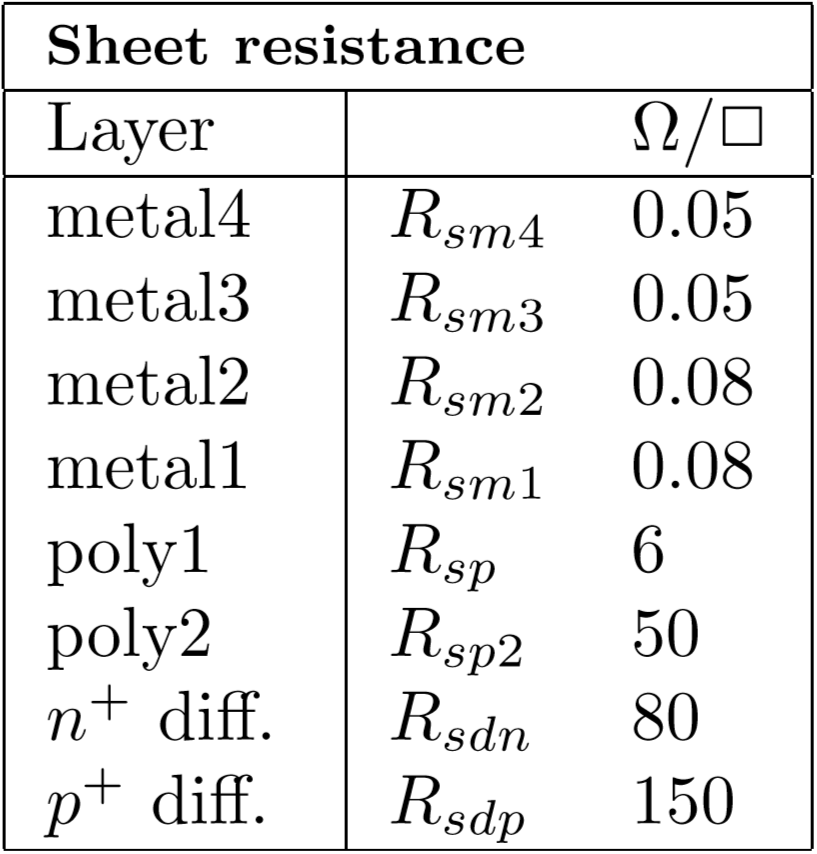
\includegraphics[keepaspectratio=true, scale=0.20]{teoricas/resistance}}
	\hspace{8mm}
	\subfloat[]{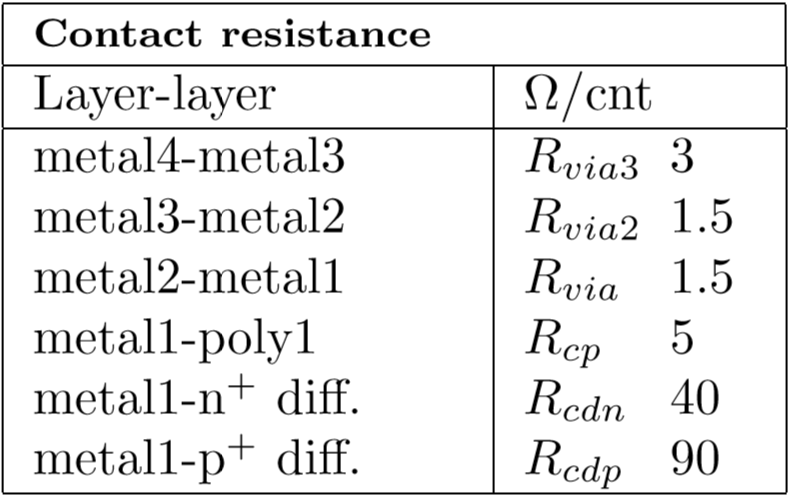
\includegraphics[keepaspectratio=true, scale=0.27]{teoricas/resistanceC}}
	\vspace{-0.8em}
\end{table}

Tomou-se a decisão de, sempre que possível, efectuar as ligações com \texttt{Metal 1} na horizontal e com \texttt{Metal 2} na vertical. Procura-se aplicar esta \textit{rule of thumb} sempre que possível, sendo que apenas não é cumprida quando se verifica que acaba por tornar mais difícil o \textit{design} do \textit{layout} ou que conduz a uma área maior porque é necessário ajustar o espaçamento entre transístores para acomodar uma ligação em \texttt{Metal 1} ou \texttt{Metal 2} consoante o caso.

Para ligar \texttt{Metal 1} a \texttt{Metal 2} é usada uma via. De referir que, optou-se também, sempre que possível, por colocar vias e contactos duplos, para que houvesse um de \textit{backup}. À semelhança do que se referiu anteriormente, isto é feito quando não dificulta o \textit{design} do \textit{layout}.

\subsubsection{Estrutura \textit{common centroid} \#1}

Relembrando a estrutura da Figura \ref{fig:common centroid}(a), a sua primeira implementação no Cadence foi feita da seguinte maneira:

\begin{figure}[H]
	\centering
	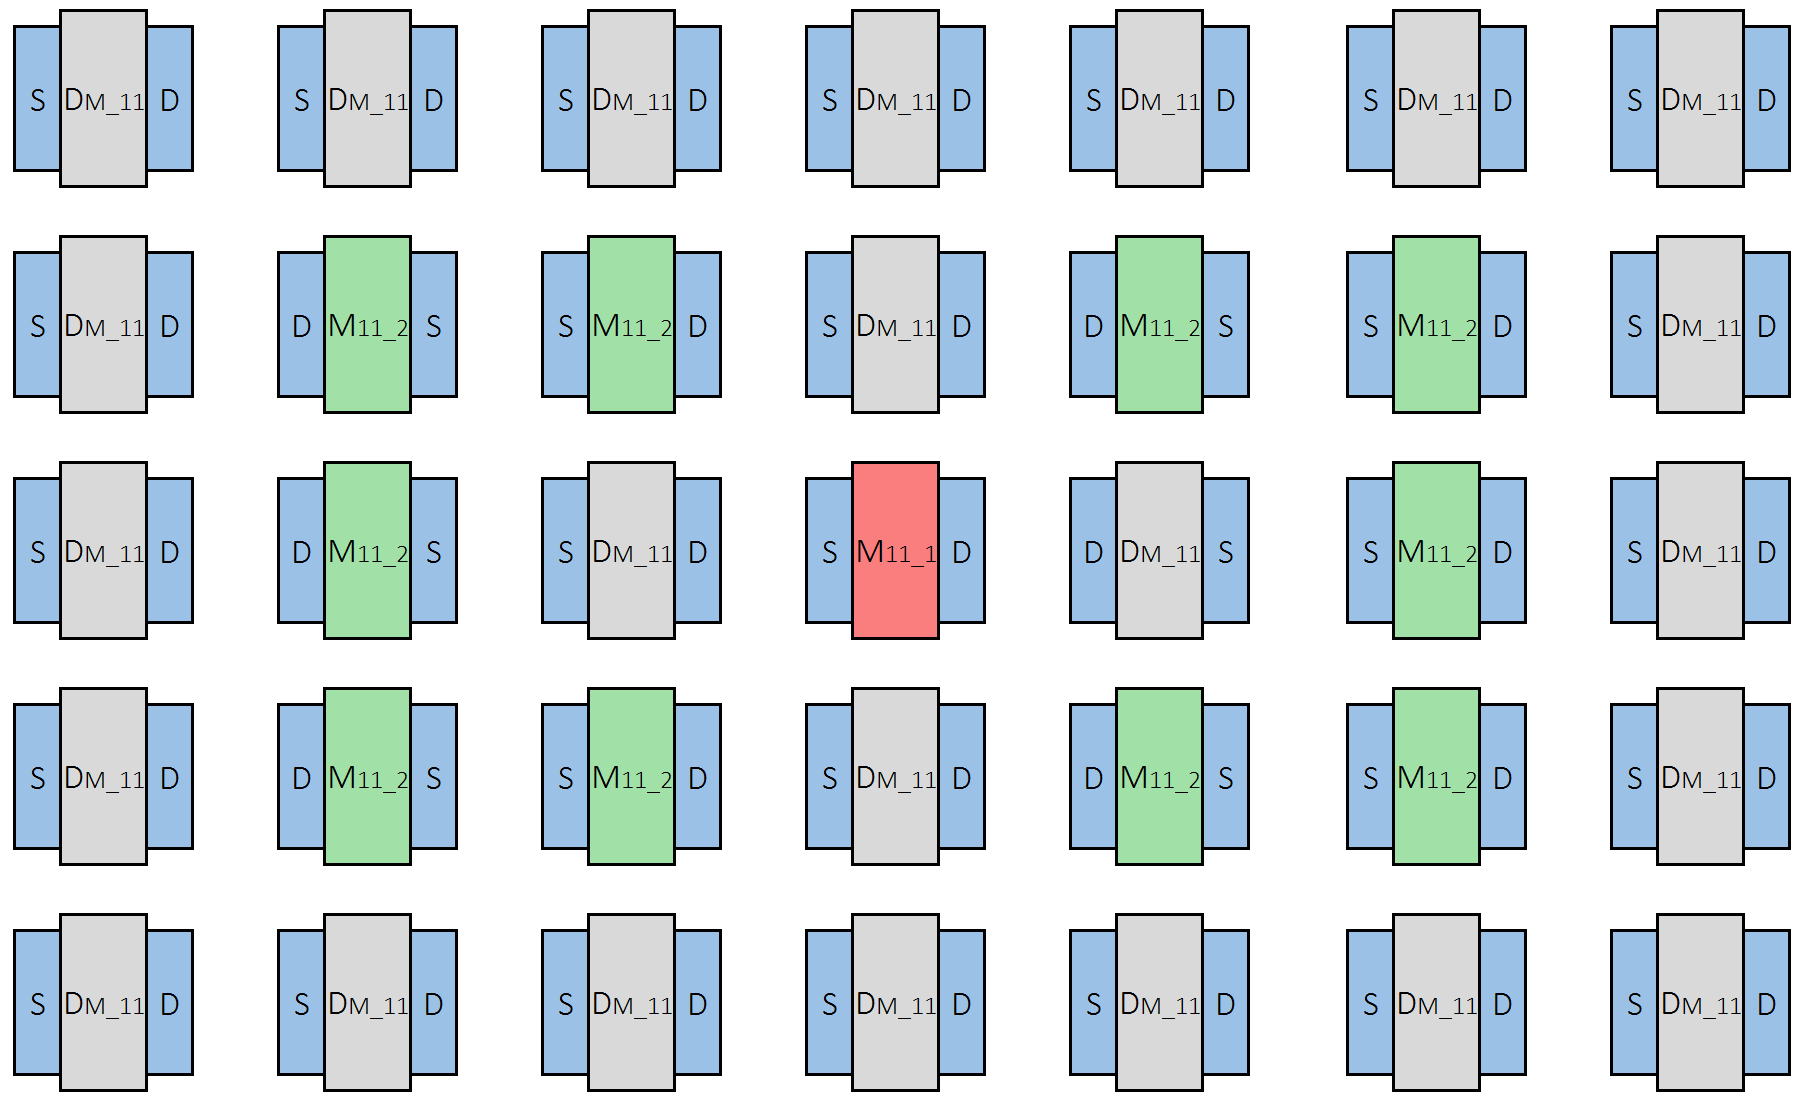
\includegraphics[keepaspectratio=true, scale=0.30]{teoricas/layout/cc1_1}
	\vspace{-0.5em}
	\caption{Esquema inicial do \textit{layout}.}
	\vspace{-0.8em} 
\end{figure}

Como se pode ver, da maneira como a estrutura \textit{common centroid} foi definida é possível sobrepor as difusões de \textit{source} dos transístores M\textsubscript{11\textsubscript{2}}, poupando assim área. Da mesma maneira, pode-se também sobrepor a \textit{source} do transístor M\textsubscript{11\textsubscript{2}} do meio com a \textit{source} do transístor \textit{dummy} que se encontra próximo do transístor M\textsubscript{11\textsubscript{1}}. Desta maneira, o circuito fica com a seguinte estrutura:

\begin{figure}[H]
	\centering
	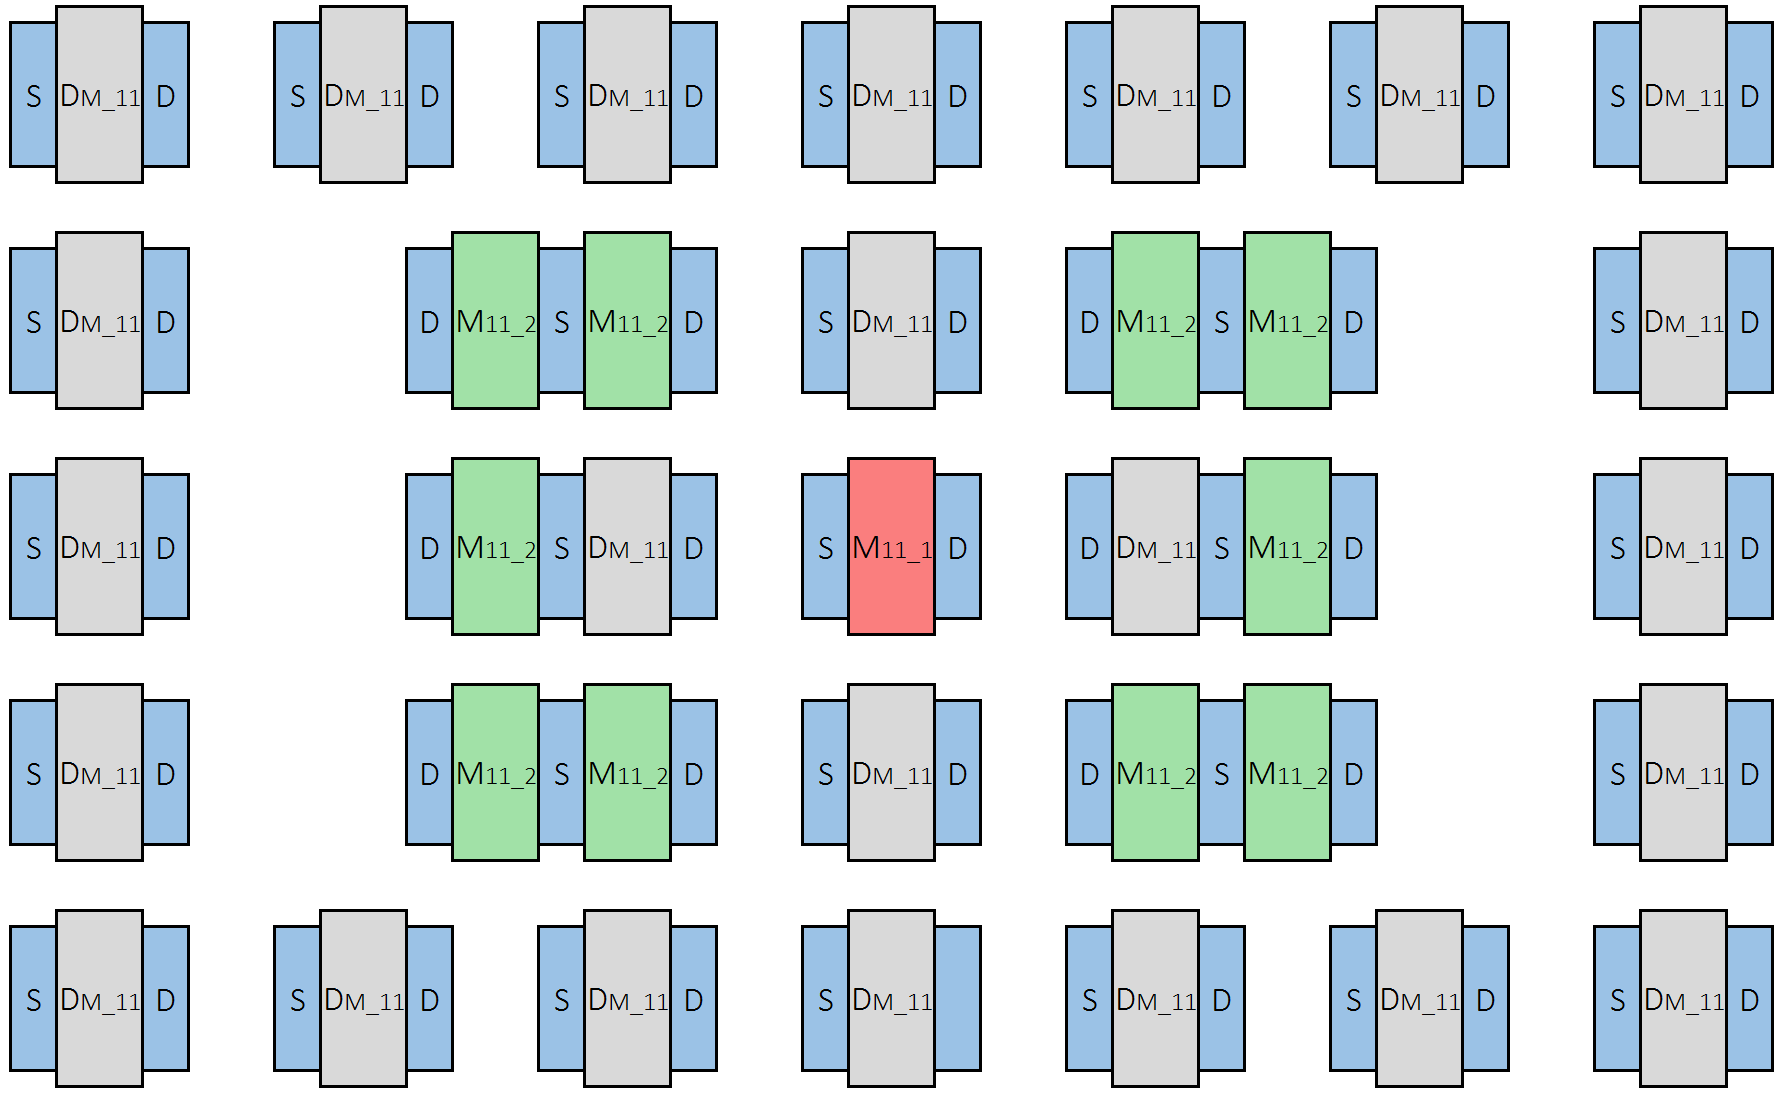
\includegraphics[keepaspectratio=true, scale=0.30]{teoricas/layout/cc1_2}
	\vspace{-0.5em}
	\caption{Estrutura resultante da agregação das difusões de alguns transístores.}
	\vspace{-0.8em} 
\end{figure}

No entanto, verifica-se que agora as vizinhanças dos transístores não estão de acordo com o pretendido, havendo ``buracos'' entre a estrutura rectangular de \textit{dummies} e a estrutura rectangular interior. Assim, optou-se por ajustar a estrutura exterior com \textit{dummies} de menores dimensões  e de modo a que a estrutura geral ficasse rectangular, apenas com o espaço necessário mínimo entre transístores que garante um correcto funcionamento do circuito.

\begin{figure}[H]
	\centering
	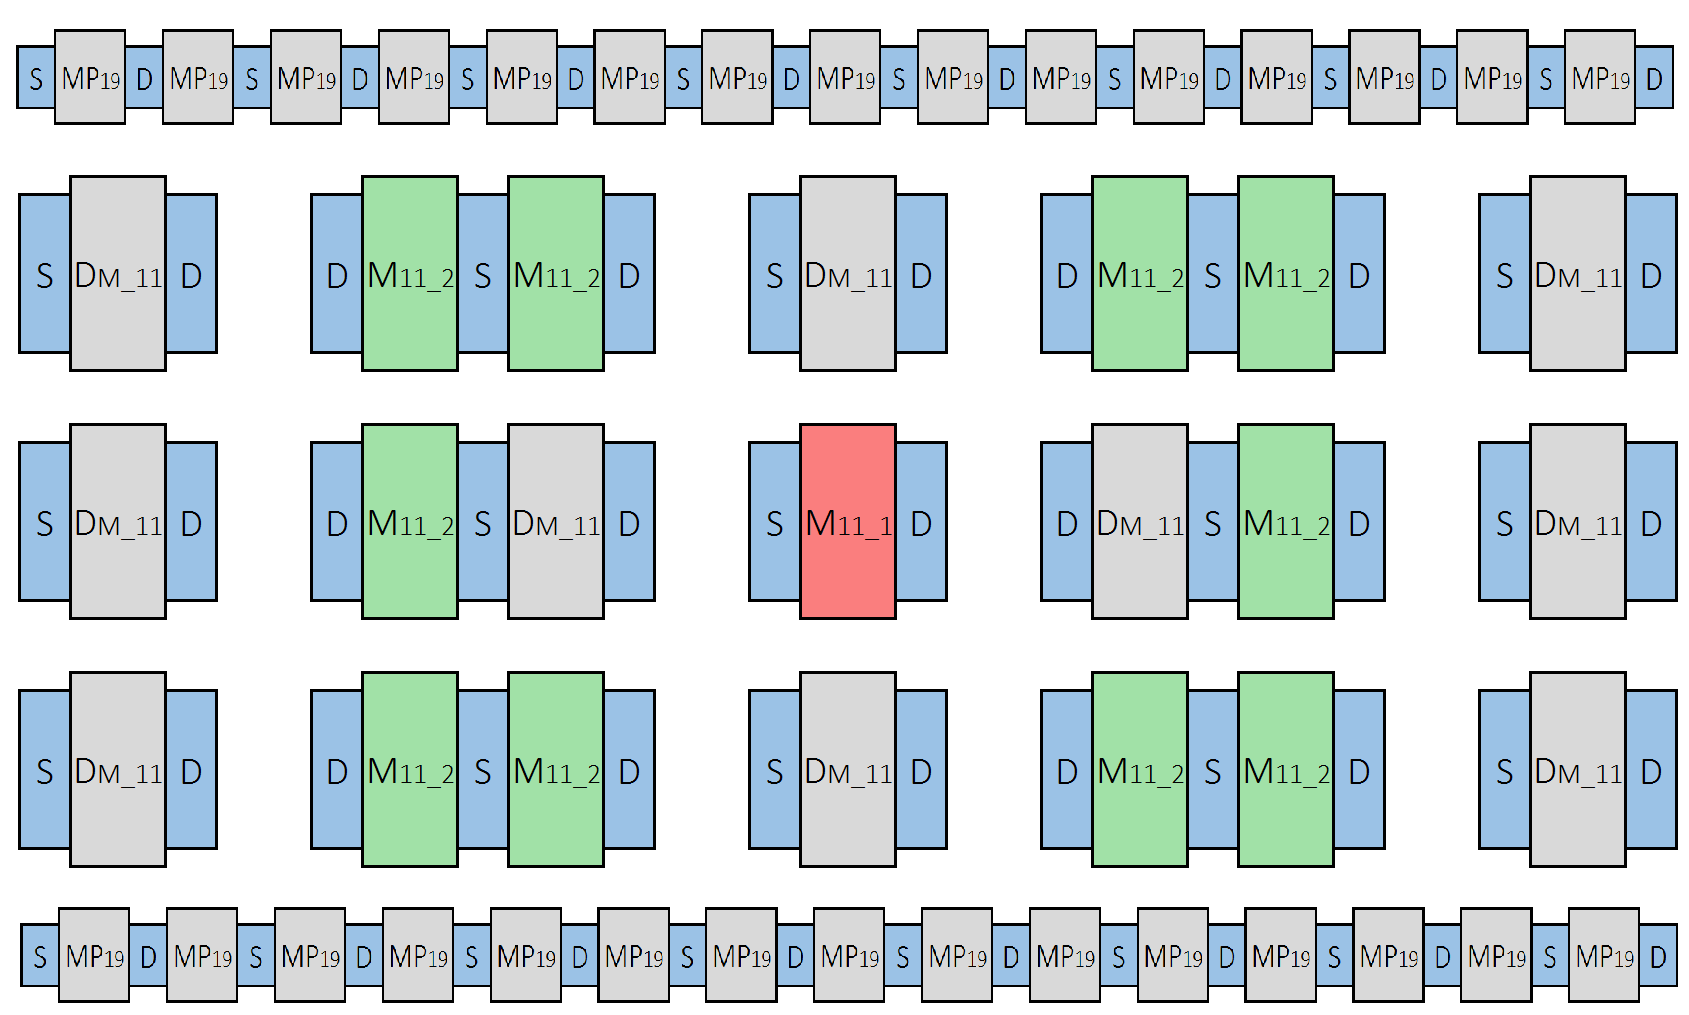
\includegraphics[keepaspectratio=true, scale=0.30]{teoricas/layout/cc1_3}
	\vspace{-0.5em}
	\caption{Estrutura resultante do \textit{layout} do espelho de corrente básico que é polarizado em corrente com $I_{BIAS}$.}
	\vspace{-0.8em} 
\end{figure} 

A implementação desta estrutura no Cadence é apresentada de seguida.

\begin{figure}[H]
	\centering
	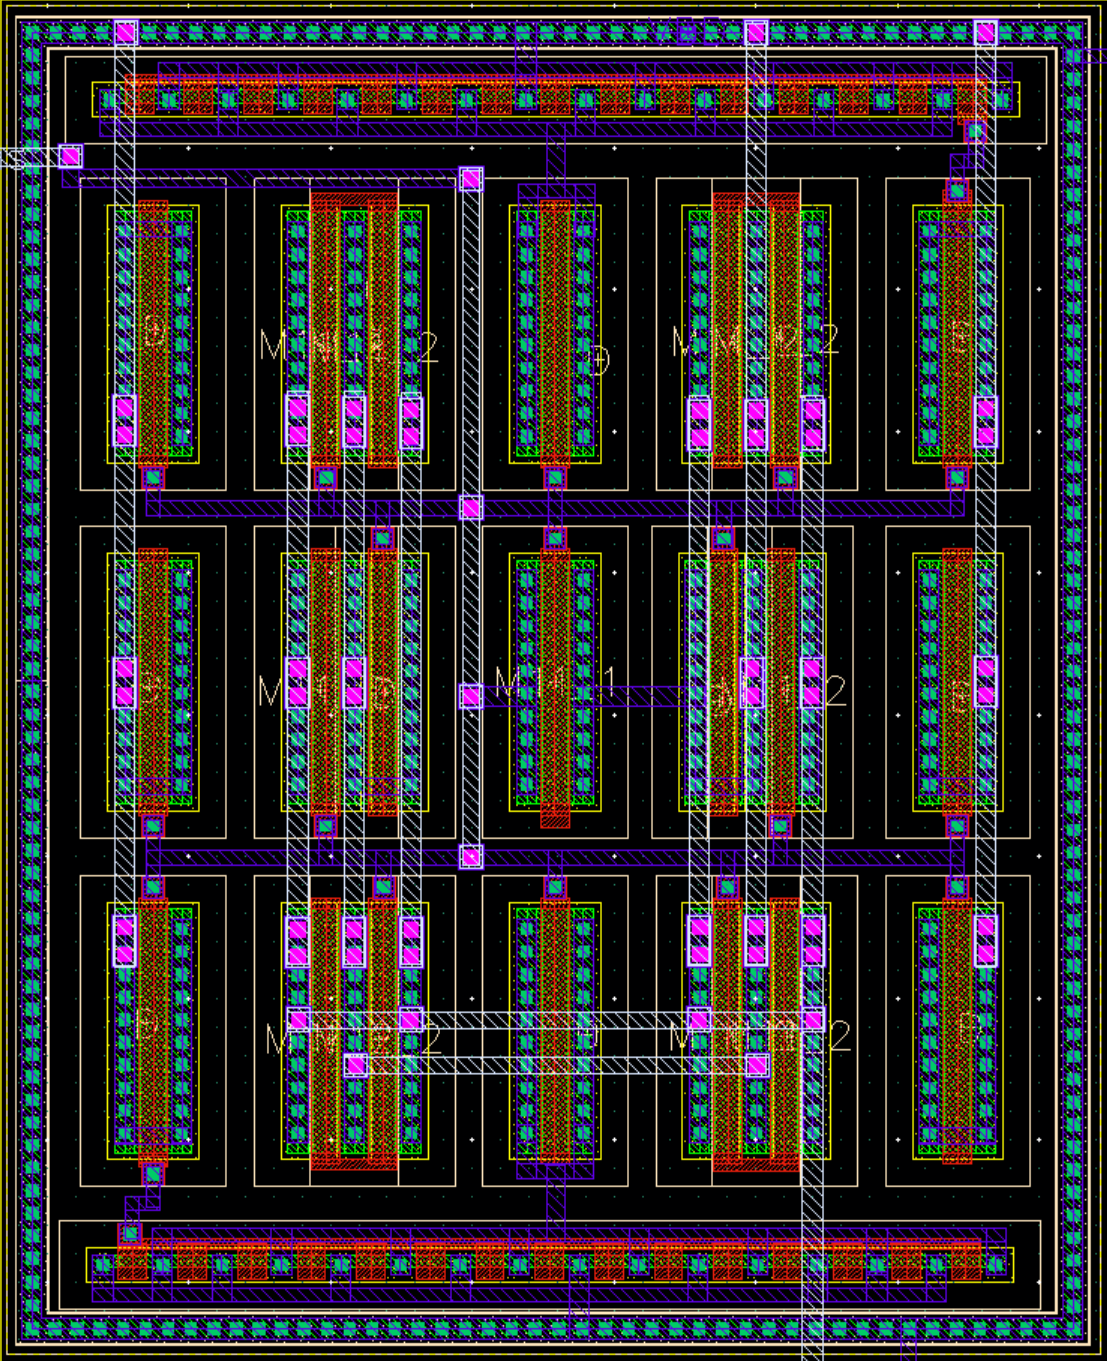
\includegraphics[keepaspectratio=true, scale=0.65]{exps/layout/espelhodecorrente}
	\vspace{-0.5em}
	\caption{\textit{Layout} da estrutura que corresponde ao espelho de corrente básico que é polarizado em corrente com $I_{BIAS}$.}
	\vspace{-0.8em}
\end{figure}

Como se pode ver, as \textit{gates} dos transístores \textit{dummy} foram ligadas a $I_{BIAS}$ e não a VDD, como seria esperado, para fazer curto-circuito aos \textit{dummies} do tipo P. A razão pela qual se faz isto é que, ao fazer estas ligações, cria-se um condensador entre $I_{BIAS}$ e VDD como se demonstra na figura seguinte.

\begin{figure}[H]
	\centering
	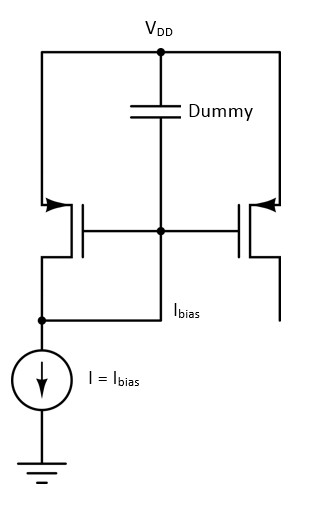
\includegraphics[keepaspectratio=true, scale=0.45]{exps/circuito_ibias}
	\vspace{-0.5em}
	\caption{Circuito que demonstra o efeito de ligar as \textit{gates} dos \textit{dummies} a $I_{BIAS}$.}
	\vspace{-0.8em}
\end{figure}

Desta forma protege-se o \textit{dummy} de variações na fonte de tensão que de outra forma iriam comprometer a integridade do transístor e como tal a do espelho de corrente, pois este condensador irá actuar como um filtro apenas aquando a ocorrência de variações.

Como se pode ver, em torno dos transístores PMOS foi colocado um poço, ou seja, aplicou-se a máscara \texttt{NTUB}. Isso tem de ser feito porque no caso dos transístores PMOS, as difusões do tipo $p$+ não podem estar directamente ligadas ao substrato, uma vez que este é do tipo $p+$. Assim, é necessário criar um poço do tipo $n$ entre as difusões e o substrato.

É de referir que dentro do poço encontra-se um \textit{guard ring} do tipo \texttt{ndiff\_ntub}. Através deste é possível polarizar o substrato a VDD, colocando sobre o \textit{guard ring} o \textit{pin} correspondente, como se pode ver na figura seguinte. 

\begin{figure}[H]
	\centering
	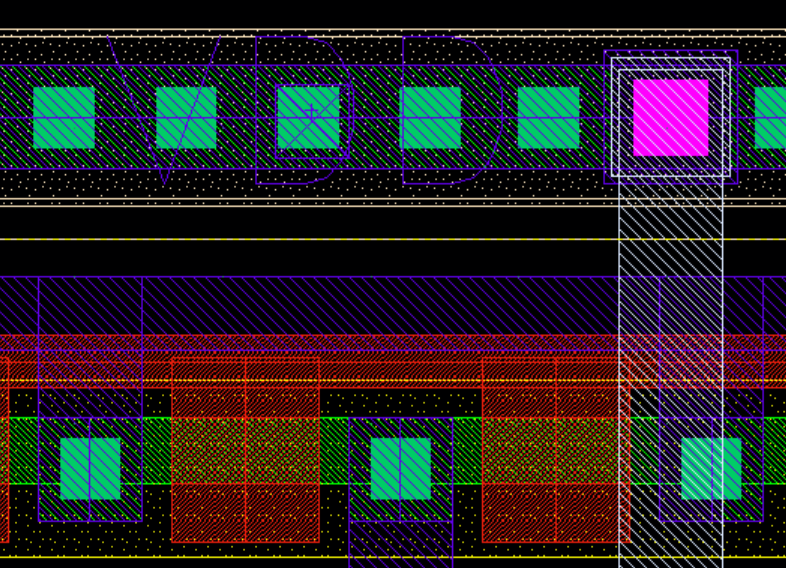
\includegraphics[keepaspectratio=true, scale=0.25]{exps/layout/pinVDD}
	\vspace{-0.5em}
	\caption{Colocação do \textit{pin} de VDD sobre o \textit{guard ring}.}
	\vspace{-0.8em}
\end{figure}

O \textit{guard ring} tem também o intuito de proteger o circuito de correntes de dispersão e, desta maneira, o ruído do substrato encontra no \textit{guard ring} blindagem.

É de referir que nesta altura da projecção do \textit{layout} quando se efectuava um DRC e um LVS sobre o \textit{design} do circuito havia dois problemas principais - \textit{hot nwell} e mau \textit{match} entre os \textit{pins} do \textit{schematic} e do \textit{layout}. O problema de \textit{hot nwell} surge quando o substrato \todo{continuar esta parte dos erros}

\subsubsection{Estrutura \textit{common centroid} \#2}

\subsubsection{Estrutura \textit{common centroid} \#3}

\subsubsection{Estrutura \textit{common centroid} \#4}

\subsection{Ligações externas entre os blocos}

\pagebreak

\section{Conclusões}

\end{document}